% Options for packages loaded elsewhere
\PassOptionsToPackage{unicode}{hyperref}
\PassOptionsToPackage{hyphens}{url}
%
\documentclass[
]{book}
\usepackage{lmodern}
\usepackage{amssymb,amsmath}
\usepackage{ifxetex,ifluatex}
\ifnum 0\ifxetex 1\fi\ifluatex 1\fi=0 % if pdftex
  \usepackage[T1]{fontenc}
  \usepackage[utf8]{inputenc}
  \usepackage{textcomp} % provide euro and other symbols
\else % if luatex or xetex
  \usepackage{unicode-math}
  \defaultfontfeatures{Scale=MatchLowercase}
  \defaultfontfeatures[\rmfamily]{Ligatures=TeX,Scale=1}
\fi
% Use upquote if available, for straight quotes in verbatim environments
\IfFileExists{upquote.sty}{\usepackage{upquote}}{}
\IfFileExists{microtype.sty}{% use microtype if available
  \usepackage[]{microtype}
  \UseMicrotypeSet[protrusion]{basicmath} % disable protrusion for tt fonts
}{}
\makeatletter
\@ifundefined{KOMAClassName}{% if non-KOMA class
  \IfFileExists{parskip.sty}{%
    \usepackage{parskip}
  }{% else
    \setlength{\parindent}{0pt}
    \setlength{\parskip}{6pt plus 2pt minus 1pt}}
}{% if KOMA class
  \KOMAoptions{parskip=half}}
\makeatother
\usepackage{xcolor}
\IfFileExists{xurl.sty}{\usepackage{xurl}}{} % add URL line breaks if available
\IfFileExists{bookmark.sty}{\usepackage{bookmark}}{\usepackage{hyperref}}
\hypersetup{
  pdftitle={Elk River Fish Passage},
  pdfauthor={Al Irvine, R.P.Bio.},
  hidelinks,
  pdfcreator={LaTeX via pandoc}}
\urlstyle{same} % disable monospaced font for URLs
\usepackage{longtable,booktabs}
% Correct order of tables after \paragraph or \subparagraph
\usepackage{etoolbox}
\makeatletter
\patchcmd\longtable{\par}{\if@noskipsec\mbox{}\fi\par}{}{}
\makeatother
% Allow footnotes in longtable head/foot
\IfFileExists{footnotehyper.sty}{\usepackage{footnotehyper}}{\usepackage{footnote}}
\makesavenoteenv{longtable}
\usepackage{graphicx,grffile}
\makeatletter
\def\maxwidth{\ifdim\Gin@nat@width>\linewidth\linewidth\else\Gin@nat@width\fi}
\def\maxheight{\ifdim\Gin@nat@height>\textheight\textheight\else\Gin@nat@height\fi}
\makeatother
% Scale images if necessary, so that they will not overflow the page
% margins by default, and it is still possible to overwrite the defaults
% using explicit options in \includegraphics[width, height, ...]{}
\setkeys{Gin}{width=\maxwidth,height=\maxheight,keepaspectratio}
% Set default figure placement to htbp
\makeatletter
\def\fps@figure{htbp}
\makeatother
\setlength{\emergencystretch}{3em} % prevent overfull lines
\providecommand{\tightlist}{%
  \setlength{\itemsep}{0pt}\setlength{\parskip}{0pt}}
\setcounter{secnumdepth}{5}
\usepackage{booktabs}
\usepackage{amsthm}
\makeatletter
\def\thm@space@setup{%
  \thm@preskip=8pt plus 2pt minus 4pt
  \thm@postskip=\thm@preskip
}
\makeatother
\usepackage{booktabs}
\usepackage{longtable}
\usepackage{array}
\usepackage{multirow}
\usepackage{wrapfig}
\usepackage{float}
\usepackage{colortbl}
\usepackage{pdflscape}
\usepackage{tabu}
\usepackage{threeparttable}
\usepackage{threeparttablex}
\usepackage[normalem]{ulem}
\usepackage{makecell}
\usepackage[]{natbib}
\bibliographystyle{apalike}

\title{Elk River Fish Passage}
\author{Al Irvine, R.P.Bio.}
\date{2020-12-14}

\begin{document}
\maketitle

{
\setcounter{tocdepth}{1}
\tableofcontents
}
\begin{verbatim}
## Reading layer `hab_wshds_ltree' from data source `C:\Users\allan\OneDrive\New_Graph\Current\2020-025_cwf_elk\scripts\fish_passage_elk_2020_reporting_cwf\data\fishpass_mapping.gpkg' using driver `GPKG'
## Simple feature collection with 7 features and 2 fields
## geometry type:  POLYGON
## dimension:      XY
## bbox:           xmin: 1778770 ymin: 541240.2 xmax: 1806472 ymax: 631526.5
## projected CRS:  NAD83 / BC Albers
## Reading layer `hab_wshds_ltree_up1' from data source `C:\Users\allan\OneDrive\New_Graph\Current\2020-025_cwf_elk\scripts\fish_passage_elk_2020_reporting_cwf\data\fishpass_mapping.gpkg' using driver `GPKG'
## Simple feature collection with 6 features and 2 fields
## geometry type:  MULTIPOLYGON
## dimension:      XY
## bbox:           xmin: 1779095 ymin: 542126.3 xmax: 1802742 ymax: 631526.5
## projected CRS:  NAD83 / BC Albers
\end{verbatim}

\begin{verbatim}
## Reading layer `hab_wshds_ltree' from data source `C:\Users\allan\OneDrive\New_Graph\Current\2020-025_cwf_elk\scripts\fish_passage_elk_2020_reporting_cwf\data\fishpass_mapping.gpkg' using driver `GPKG'
## Simple feature collection with 7 features and 2 fields
## geometry type:  POLYGON
## dimension:      XY
## bbox:           xmin: 1778770 ymin: 541240.2 xmax: 1806472 ymax: 631526.5
## projected CRS:  NAD83 / BC Albers
## Reading layer `hab_wshds_ltree_up1' from data source `C:\Users\allan\OneDrive\New_Graph\Current\2020-025_cwf_elk\scripts\fish_passage_elk_2020_reporting_cwf\data\fishpass_mapping.gpkg' using driver `GPKG'
## Simple feature collection with 6 features and 2 fields
## geometry type:  MULTIPOLYGON
## dimension:      XY
## bbox:           xmin: 1779095 ymin: 542126.3 xmax: 1802742 ymax: 631526.5
## projected CRS:  NAD83 / BC Albers
\end{verbatim}

\hypertarget{executive-summary}{%
\chapter*{Executive Summary}\label{executive-summary}}
\addcontentsline{toc}{chapter}{Executive Summary}

\hypertarget{intro}{%
\chapter{Introduction}\label{intro}}

New Graph Environment was retained by the Canadian Wildlife Federation in the fall of 2020 to conduct fish passage assessments of stream crossings within the Elk River watershed upstream of the Elko Dam near Elko, BC. The work was carried out in accordance with the BC Ministry of Environment: Field Assessment for Determining Fish Passage at Closed Bottom Structures, 4th Edition \citep{fish_passage_assessments} and Fish Passage Strategic Approach: Protocol for Prioritizing Sites for Fish Passage Remediation: 4th Edition \citep{fishpassagetechnicalworkinggroupFishPassageStrategic2014}.

The health and viability of freshwater fish populations can depend on access to tributary and off channel areas which provide refuge during high flows, opportunities for foraging, overwintering habitat, spawning habitat and summer rearing habitat \citep{Bramblett_2002, swalesRoleOffChannelPonds1989}. Culverts can present barriers to fish migration due to increased water velocity, turbulence, a vertical drop at the culvert outlet and/or maintenance issues \citep{slaneyFishHabitatRehabilitation1997}. Reconnection of fragmented habitats is a management action that can generate some of the highest ecological returns on economic investments relative to other habitat restoration techniques \citep{saldicaromileStreamHabitatRestoration2004}.

\hypertarget{background}{%
\chapter{Background}\label{background}}

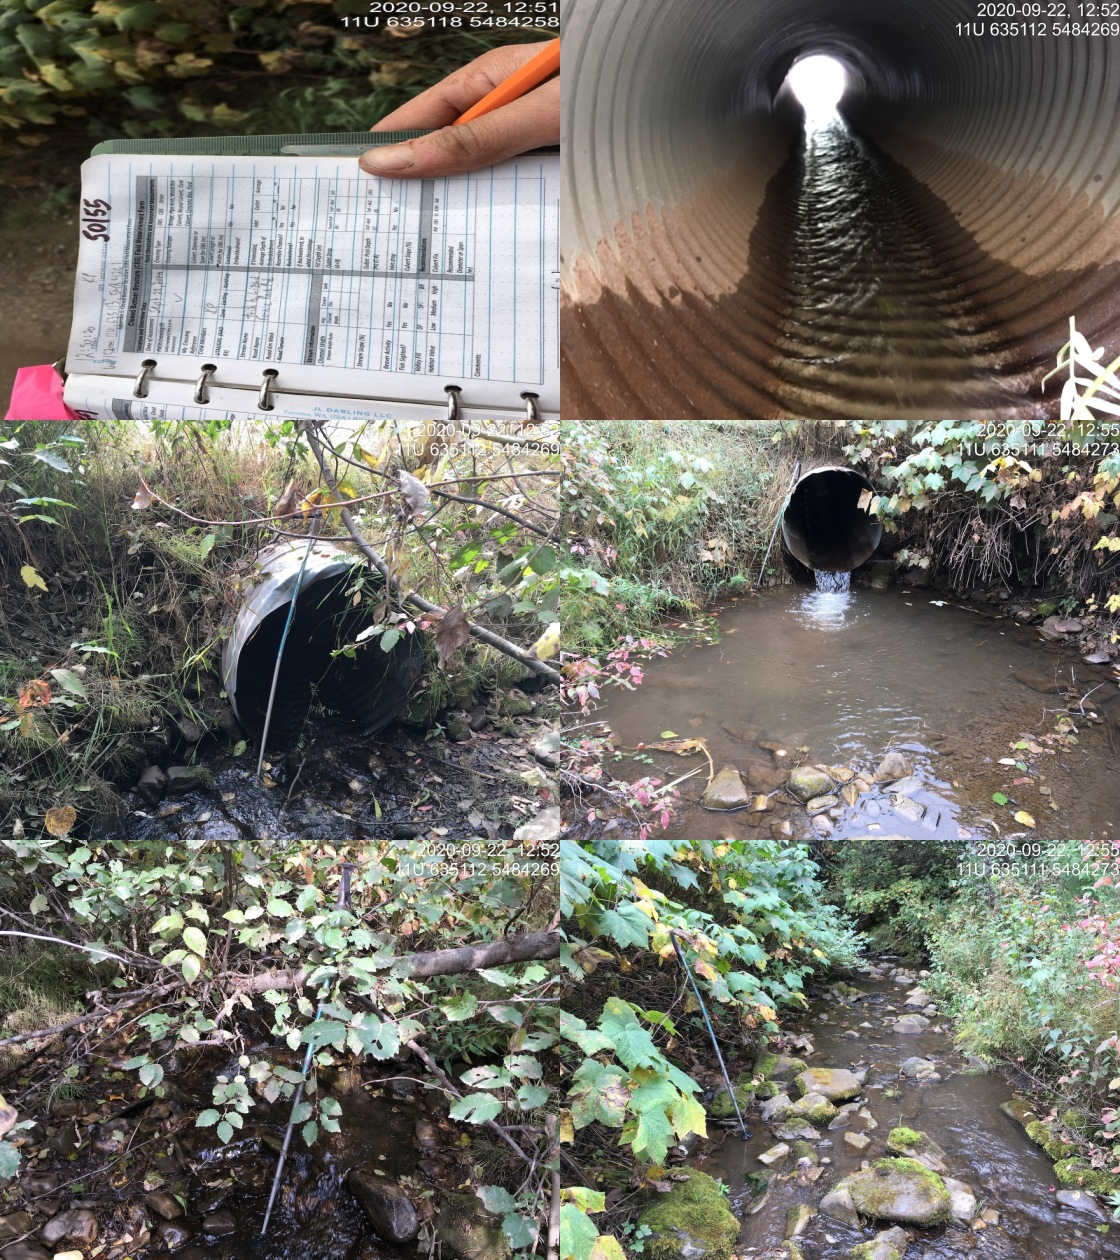
\includegraphics[width=15.56in]{data/photos/50155/crossing_all}

As a result of high-level direction from the provincial government, a Fish Passage Strategic Approach protocol has been developed for British Columbia to ensure that the greatest opportunities for restoration of fish passage are pursued. A Fish Passage Technical Working Group has been formed to coordinate the protocol and data is continuously amalgamated within the Provincial Steam Crossing Inventory System (PSCIS). The strategic approach protocol involves a four-phase process as described in \citet{fishpassagetechnicalworkinggroupFishPassageStrategic2014} :

\begin{itemize}
\tightlist
\item
  Phase 1: Fish Passage Assessment -- Fish stream crossings within watersheds with high fish values are assessed to determine barrier status of structures and document a general assessment of adjacent habitat quality and quantity.
\item
  Phase 2: Habitat Confirmation -- Assessments of crossings prioritized for follow up in Phase 1 studies are conducted to confirm quality and quantity of habitat upstream and down as well as to scope for other potential nearby barriers that could affect the practicality of remediation.
\item
  Phase 3: Design -- Site plans and designs are drawn for priority crossings where high value fish habitat has been confirmed.
\item
  Phase 4: Remediation -- Reconnection of isolated habitats through replacement, rehabilitation or removal of prioritized crossing structure barriers.
\end{itemize}

The scope of 2020/2021 project activities reported on in this document includes planning for and implementation of the first phase of fish passage assessment in the Elk River watershed upstream of the Elko Dam.

\hypertarget{project-location}{%
\section{Project Location}\label{project-location}}

The project was focused within the upper Elk River watershed upstream of the Elko Dam located at Elko, BC.

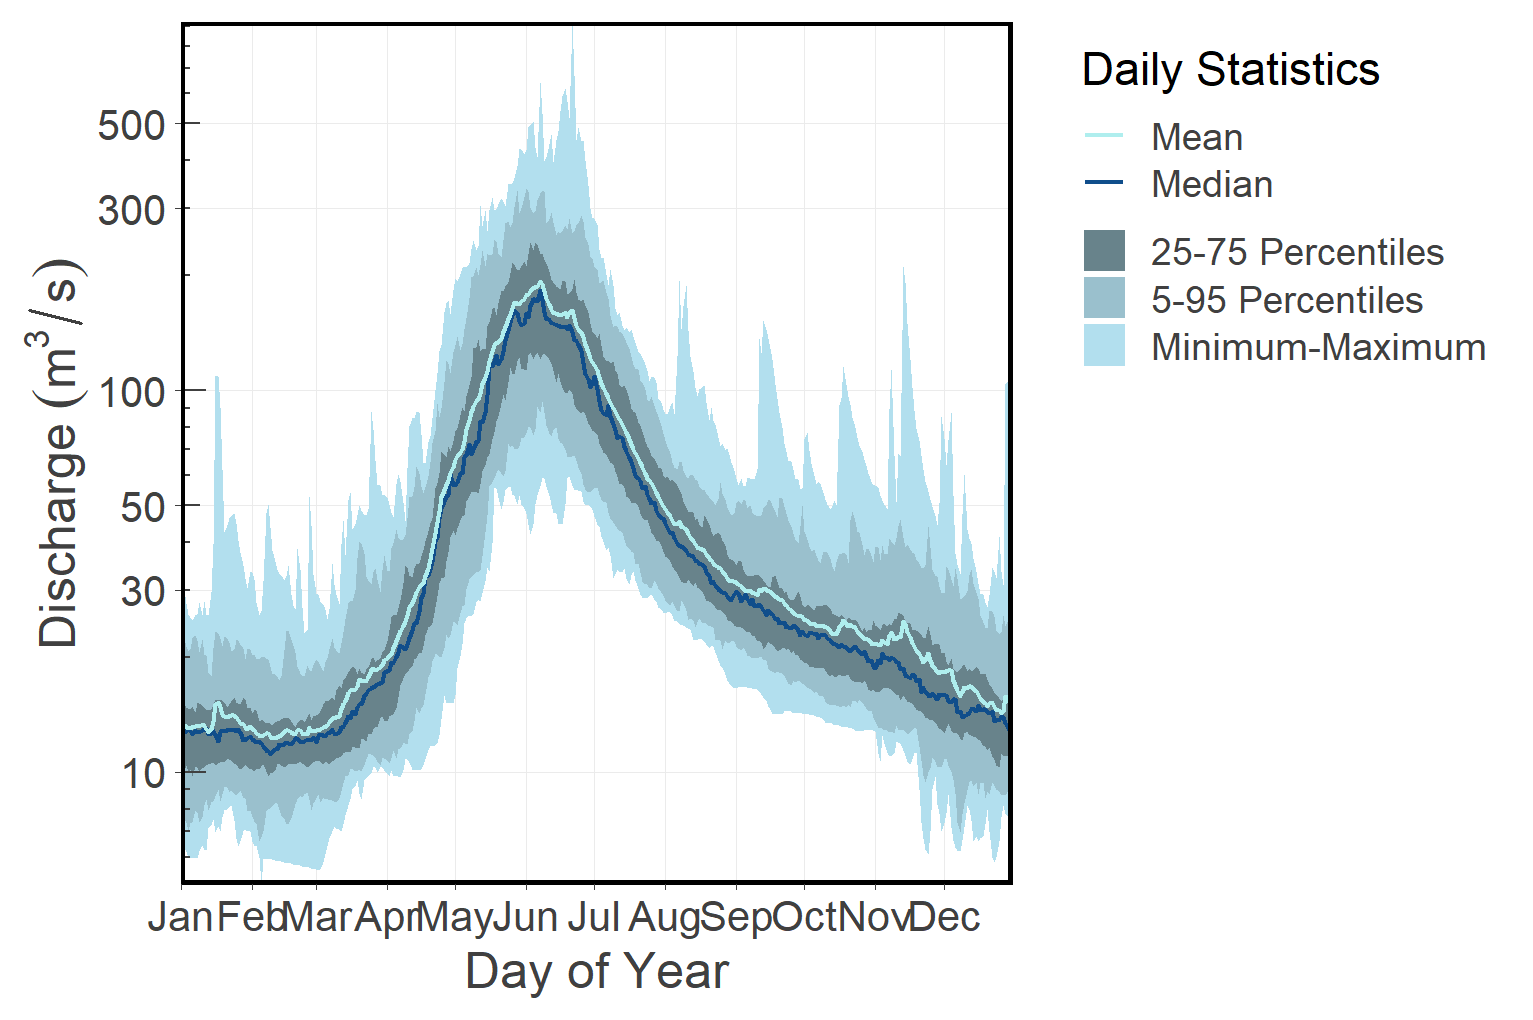
\includegraphics{fig/hydrology1.png}

\hypertarget{fisheries}{%
\section{Fisheries}\label{fisheries}}

\hypertarget{methods}{%
\chapter{Methods}\label{methods}}

\hypertarget{planning}{%
\section{Planning}\label{planning}}

We produced detailed maps of the project area identifying all locations where 1:20,000 scale TRIM map streams where intersected with roads. To determine target field sites we reviewed background habitat confirmation reports from \citep{masseEKConfirmation2015}

which crossings on fish habitat with significant quantities of fish habitat upstream had not yet been assessed, we used the Fish Habitat Model to the estimate the quantity and quality of fish habitat potentially upstream of crossings. Using the criteria below we screen previously cross reference modelled crossing locations with sites already within the Provincial Stream Crossing Summary System. Target crossings were identified as previously unnassessed crossings on streams with likely significant quantities of fish habitat upstream.

\hypertarget{fish-passage-assessments}{%
\section{Fish Passage Assessments}\label{fish-passage-assessments}}

In the field, crossings surveyed included closed bottom structures (CBS), open bottom structures (OBS) and crossings considered ``other'' (fords, weirs, etc.). Six digit numerical crossing identifiers were generated for each crossings modeled. Crossings identified in the field that had no corresponding GIS generated ID were given unique identifiers beginning with the date in YYYYMMDD format appended with an identifier between 1 and 10 (ex. 2020091601). Photos were taken at surveyed crossings and when possible included images of the road, crossing inlet, crossing outlet, crossing barrel, channel downstream and channel upstream of the crossing and any relevant features. Additionally, the following information was recorded for all surveyed crossings: date of inspection, crossing reference, crew member initials, Universal Transverse Mercator (UTM) coordinates, stream name, road name and kilometer, road tenure information, crossing type, crossing subtype, culvert diameter or span for OBS, culvert length or width for OBS. A more detailed ``full assessment'' was completed for all closed bottom structures.

Full assessments also included the following parameters: presence/absence of continuous culvert embedment (yes/no), average depth of embedment, whether or not the culvert bed resembled the native stream bed, presence of and percentage backwatering, fill depth, outlet drop, outlet pool depth, inlet drop, culvert slope, average downstream channel width, stream slope, presence/absence of beaver activity, presence/absence of fish at time of survey, type of valley fill, and a habitat value rating. Habitat value ratings were based on channel morphology, flow characteristics (perennial, intermittent, ephemeral), fish migration patterns, the presence/absence of deep pools, un-embedded boulders, substrate, woody debris, undercut banks, aquatic vegetation and overhanging riparian vegetation (Table \ref{tab:tab-hab-value}). For crossings determined to be potential barriers or barriers based on the data (see section 2.3.2), a culvert fix and recommended diameter/span was proposed.

All field data collected including photos were uploaded to the Provincial Stream Crossing Inventory System (PSCIS).

\begin{table}

\caption{\label{tab:tab-hab-value}Habitat value criteria (Fish Passage Technical Working Group, 2011).}
\centering
\begin{tabu} to \linewidth {>{}l>{\raggedright}X}
\hline
Habitat Value & Fish Habitat Criteria\\
\hline
High & The presence of high value spawning or rearing habitat (e.g., locations with abundance of suitably sized gravels, deep pools, undercut banks, or stable debris) which are critical to the fish population.\\
\hline
Medium & Important migration corridor. Presence of suitable spawning habitat. Habitat with moderate rearing potential for the fish species present.\\
\hline
Low & No suitable spawning habitat, and habitat with low rearing potential (e.g., locations without deep pools, undercut banks, or stable debris, and with little or no suitably sized spawning gravels for the fish species present).\\
\hline
\end{tabu}
\end{table}

\hypertarget{barrier-scoreing}{%
\section{Barrier Scoreing}\label{barrier-scoreing}}

Fish passage potential was determined for each stream crossing identified as a closed bottom structure on fish bearing and potentially fish bearing stream reaches. The combined scores from five criteria: depth and degree to which the structure is embedded, outlet drop, stream width ratio, culvert slope, and culvert length were used to screen whether each culvert was a likely barrier to some fish species and life stages (Table \ref{tab:tab-barrier-scoring}, Table \ref{tab:tab-barrier-result}. These criteria were developed based on data obtained from various studies and reflect an estimation for the passage of a juvenile salmon or small resident rainbow trout \citetext{\citealp[ ]{clarkinNationalInventoryAssessment2005}; \citealp{bellFisheriesHandbookEngineering1991}; \citealp{thompsonAssessingFishPassage2013}}.

\begin{table}

\caption{\label{tab:tab-barrier-scoring}Fish Barrier Scoring (Fish Passage Technical Working Group 2011).}
\centering
\resizebox{\linewidth}{!}{
\begin{tabular}[t]{l|l|l|l|l|l|l|l|l|l|l}
\hline
\textbf{Risk} & \textbf{Embedded} & \textbf{Value} & \textbf{Outlet Drop (cm)} & \textbf{Value} & \textbf{SWR} & \textbf{Value} & \textbf{Slope (\%)} & \textbf{Value} & \textbf{Length (m)} & \textbf{Value}\\
\hline
LOW & >30cm or >20\% of diameter and continuous & 0 & <15 & 0 & <1.0 & 0 & <1 & 0 & <15 & 0\\
\hline
MOD & <30cm or 20\% of diameter but continuous & 5 & 15-30 & 5 & 1.0-1.3 & 3 & 1-3 & 5 & 15-30 & 3\\
\hline
HIGH & No embedment or discontinuous & 10 & >30 & 10 & >1.3 & 6 & >3 & 10 & >30 & 6\\
\hline
\end{tabular}}
\end{table}

\begin{table}

\caption{\label{tab:tab-barrier-result}Fish Barrier Scoring Results (Fish Passage Technical Working Group 2011).}
\centering
\begin{tabular}[t]{l|l}
\hline
Cumlative Score & Result\\
\hline
0-14 & passable\\
\hline
15-19 & potential barrier\\
\hline
>20 & barrier\\
\hline
\end{tabular}
\end{table}

\hypertarget{cost-benefit-analysis}{%
\section{Cost Benefit Analysis}\label{cost-benefit-analysis}}

A cost benefit analysis was conducted for each crossing considered a barrier based on the amount of potential habitat to be made available by remediating fish passage at the site and an estimate of associated costs.

\hypertarget{habitat-gain-index}{%
\section{Habitat Gain Index}\label{habitat-gain-index}}

The habitat gain index is the quantity of modelled habitat upstream of the subject crossing and represents an estimate of habitat gained with remediation of fish passage at the crossing. For this project we set the threshold between fish and non-fish habitat at a gradient of 20\% representing the gradient limit accessible to downstream populations. A ``net'' value for the index used meaning that if there is a documented PSCIS barrier crossing upstream of the subject crossing or a modelled unassessed crossing the amount of habitat is totaled to that point.

Potential options to remediate fish passage included: removal of the structure, backwatering

Cost estimates for structure replacement were generated based on the channel width, slope of the culvert, depth of fill and the road type. Base costs for installation of bridges and embedded culverts were estimated based on interviews with Phil MacDonald, Engineering Specialist FLNR - Kootenay and Steve Page, Area Engineer - FLNR - Northern Engineering Group. Costs for installation of bridges on forest service roads was estimated at \$12.5K/m and assumes that the road can be closed during construction. For streams with channel widths \textless2m embedded culverts can be effective with installation costs estimated at \$25k

\hypertarget{results}{%
\chapter{Results}\label{results}}

\hypertarget{phase-1}{%
\section{Phase 1}\label{phase-1}}

A total of XXX assessments were conducted between xxx and xxxxxxxxxx. Site details and photos are presented in

The analysis phase is summarized in Table \ref{tab:cost-est} {[}test{]}{[}test{]}

\begin{table}

\caption{\label{tab:cost-est}Modelled upstream habitat estimate and cost benefit.}
\centering
\fontsize{11}{13}\selectfont
\begin{tabu} to \linewidth {>{\raggedleft}X>{\raggedright}X>{\raggedright}X>{\raggedleft}X>{\raggedright}X>{\raggedright}X>{\raggedleft}X>{\raggedleft}X>{\raggedleft}X>{\raggedleft}X}
\hline
External ID & Stream & Road & Stream Width (m) & Priority & Fix & Cost Est ( \$K) & Habitat Upstream (m) & Cost Benefit (m / \$K) & Cost Benefit (m2 / \$K)\\
\hline
4600026 & Tributary to Elk River & Dicken Rd & 2.20 & low & OBS & 250 & 225 & 0.9 & 1.0\\
\hline
4600028 & Bean Creek & Dicken Rd & 2.00 & mod & OBS & 250 & 404 & 1.6 & 1.6\\
\hline
4600037 & Dalzell Creek & Driveway & 2.50 & low & OBS & 750 & 264 & 0.4 & 0.4\\
\hline
4600038 & Dalzell Creek & Driveway & 1.20 & low & SS-CBS & 150 & 1294 & 8.6 & 5.2\\
\hline
4600039 & Dalzell Creek & Lower Elk Valley Road & 3.80 & low & OBS & 750 & 206 & 0.3 & 0.5\\
\hline
4600069 & Weigart Creek & Highway 43 & 4.30 & high & OBS & 2500 & 1206 & 0.5 & 1.0\\
\hline
4600070 & Brule Creek & Highway 43 & 6.10 & high & OBS & 3050 & 763 & 0.3 & 0.8\\
\hline
4600080 & Tributary to Elk River & Cokato Road & 2.10 & low & OBS & 250 & 748 & 3.0 & 3.1\\
\hline
4600084 & Littlemoor Creek & Lower Elk Valley Road & 1.00 & low & SS-CBS & 150 & 145 & 1.0 & 0.5\\
\hline
4600090 & Tributary to Elk River & Lower Elk Valley Road & 0.00 & low & SS-CBS & 150 & 620 & 4.1 & 0.0\\
\hline
4600092 & North Littlemoor Creek & Lower Elk Valley Road & 1.50 & low & SS-CBS & 150 & 635 & 4.2 & 3.2\\
\hline
4600102 & Tributary to Elk River & McGiverin Road & 0.50 & low & SS-CBS & 25 & 471 & 18.8 & 4.7\\
\hline
4600130 & Tributary to Elk River & Cokato Road & 0.65 & low & SS-CBS & 50 & 94 & 1.9 & 0.6\\
\hline
4600134 & Tributary to Elk River & Fernie ski hill & 1.40 & low & SS-CBS & 25 & 58 & 2.3 & 1.6\\
\hline
4600140 & Whiting Creek & Highway 43 & 0.60 & low & SS-CBS & 150 & 569 & 3.8 & 1.1\\
\hline
4600158 & Bean Creek & Highway 3 & 3.20 & mod & OBS & 2500 & 1772 & 0.7 & 1.1\\
\hline
4600169 & Tributary to Elk River & Highline Drive (Fernie ski hill) & 2.30 & mod & OBS & 475 & 219 & 0.5 & 0.5\\
\hline
4600181 & Tributary to Elk River & Line creek mine road & 0.50 & low & SS-CBS & 50 & 492 & 9.8 & 2.5\\
\hline
4600183 & Brule Creek & Busato Road & 7.10 & high & OBS & 178 & 128 & 0.7 & 2.6\\
\hline
4600184 & North Littlemoor Creek & Highway 43 & 1.60 & mod & SS-CBS & 500 & 533 & 1.1 & 0.9\\
\hline
4600185 & Littlemoor Creek & Highway 43 & 1.20 & mod & SS-CBS & 500 & 2508 & 5.0 & 3.0\\
\hline
4600186 & Hollow Creek & Highway 43 & 1.10 & low & SS-CBS & 500 & 0 & 0.0 & 0.0\\
\hline
4600316 & Tributary to Elk River & Cokato Road & 4.10 & low & OBS & 250 & 36 & 0.1 & 0.3\\
\hline
4600329 & Tributary to Whiting Creek & Lower Elk Valley Road & 0.50 & low & SS-CBS & 150 & 273 & 1.8 & 0.5\\
\hline
4600332 & Tributary to Elk River & Highway 3 & 3.30 & mod & OBS & 2500 & 1616 & 0.6 & 1.1\\
\hline
4600367 & Hartley Creek & Dicken Road & 3.50 & high & OBS & 250 & 278 & 1.1 & 1.9\\
\hline
4601556 & Tributary to Elk River & Fernie ski hill & 1.30 & low & SS-CBS & 25 & 85 & 3.4 & 2.2\\
\hline
4601594 & Tributary to Elk River & Railway & 2.70 & low & OBS & 125 & 28 & 0.2 & 0.3\\
\hline
4601639 & Tributary to Elk River & Fernie ski hill & 1.50 & low & SS-CBS & 25 & 58 & 2.3 & 1.7\\
\hline
4602270 & Tributary to Grave Creek & NA & 1.50 & low & SS-CBS & 25 & 5421 & 216.8 & 162.6\\
\hline
4602349 & Tributary to Elk River & Fernie Nordic Trail & 2.00 & mod & OBS & 125 & 1747 & 14.0 & 14.0\\
\hline
4602533 & Grave Creek & NA & 0.10 & low & SS-CBS & 25 & 181 & 7.2 & 0.4\\
\hline
4603291 & Cokato Creek & Cokato Road & 4.50 & low & OBS & 250 & 688 & 2.8 & 6.2\\
\hline
4604198 & Tributary to Elk River & Hadner FSR & 2.90 & low & OBS & 162 & 0 & 0.0 & 0.0\\
\hline
4604455 & Tributary to Elk River & Fernie ski hill & 1.50 & low & SS-CBS & 25 & 58 & 2.3 & 1.7\\
\hline
4605649 & Tributary to Elk River & Elk River FSR & 1.00 & low & SS-CBS & 25 & 1504 & 60.2 & 30.1\\
\hline
4605653 & Tributary to Elk River & Elk River FSR & 2.50 & low & OBS & 125 & 2233 & 17.9 & 22.3\\
\hline
4605675 & Tributary to Elk River & Elk River FSR & 2.00 & low & OBS & 125 & 762 & 6.1 & 6.1\\
\hline
4605697 & Crossing Creek & Elk River FSR & 2.50 & low & OBS & 125 & 1481 & 11.8 & 14.8\\
\hline
4605705 & Tributary to Elk River & Elk River FSR & 1.00 & low & SS-CBS & 25 & 621 & 24.8 & 12.4\\
\hline
4605707 & Tributary to Elk River & Elk River FSR & 2.30 & low & OBS & 125 & 1178 & 9.4 & 10.8\\
\hline
4605708 & Tributary to Lowe Creek & Elk River FSR & 1.10 & low & SS-CBS & 25 & 1348 & 53.9 & 29.7\\
\hline
4605732 & Tributary to Elk River & Elk River FSR & 3.50 & high & OBS & 312 & 6845 & 21.9 & 38.4\\
\hline
4605733 & Tributary to Elk River & Elk River FSR & 3.10 & low & OBS & 125 & 2865 & 22.9 & 35.5\\
\hline
4605742 & Lowe Creek & Elk River FSR & 2.50 & mod & OBS & 125 & 6563 & 52.5 & 65.6\\
\hline
4606669 & Tributary to Elk River & Spur from Elk River FSR & 1.00 & low & RM & NA & 940 & NA & NA\\
\hline
4606835 & Tributary to Elk River & Spur from Elk River FSR & 1.00 & low & SS-CBS & 25 & 0 & 0.0 & 0.0\\
\hline
2020092303 & Tributary to Elk River & Driveway & 1.50 & low & SS-CBS & 25 & 582 & 23.3 & 17.5\\
\hline
\end{tabu}
\end{table}

\hypertarget{phase-2}{%
\section{Phase 2}\label{phase-2}}

Raw results are included in digital format as \href{https://github.com/NewGraphEnvironment/fish_passage_elk_2020_reporting/raw/master/data/habitat_confirmations.xls}{Attachment 2} and summarized in Tables \ref{tab:tab-overview} - \ref{tab:tab-habitat-summary}

\begin{table}

\caption{\label{tab:tab-overview}Overview of habitat confirmation sites.}
\centering
\fontsize{11}{13}\selectfont
\begin{tabu} to \linewidth {>{\raggedleft}X>{\raggedright}X>{\raggedright}X>{\raggedright}X>{\raggedright}X>{\raggedright}X>{\raggedleft}X>{\raggedright}X>{\raggedright}X>{\raggedright}X}
\hline
Site & Stream & Road & Tenure & UTM (11U) & Fish Species & Habitat Gain (km) & Habitat Value & Priority & Comments\\
\hline
50155 & Tributary to Lizard Creek & Island Lake Lodge Road & MoTi recreation & 635113 5484261 & NA & NA & Medium & moderate & NA\\
\hline
50159 & Tributary to Lizard Creek & Island Lake Lodge Road & MoTi recreation & 633320 5484601 & NA & NA & Medium & high & NA\\
\hline
50185 & Tributary to Morrisey Creek & River Rd & FLNR 5466 & 645683 5469025 & NA & NA & High & moderate & NA\\
\hline
62423 & Tributary to Grave Creek & Grave Creek FSR & Unknown & 660508 5524239 & NA & NA & Low & low & NA\\
\hline
62425 & Grave Creek & Spur & Canfor R08362 & 661486 5524426 & NA & NA & Medium & moderate & NA\\
\hline
62426 & Grave Creek & Spur & Canfor R08362 & 661611 5524460 & NA & NA & Medium & moderate & NA\\
\hline
62516 & Tributary to Lizard Creek & Island Lake Lodge Road & MoTi recreation & 636123 5484087 & NA & NA & Medium & moderate & Fry observed upstream and downstream\\
\hline
197533 & Brule Creek & Busato Rd & MoTi local & 651626 5528888 & NA & 0 & High & high & Deactivate\\
\hline
197555 & Tributary to Elk River & Elk River FSR & FLNR 0103 & 646735 5554534 & BT & NA & High & moderate & NA\\
\hline
197559 & Brule Creek & Highway 43 & MoTi highway & 651516 5528829 & BT, WCT & NA & Medium & moderate & NA\\
\hline
\end{tabu}
\end{table}

\begin{table}

\caption{\label{tab:unnamed-chunk-5}Summary of Phase 2 fish passage assessments.}
\centering
\fontsize{11}{13}\selectfont
\begin{tabu} to \linewidth {>{\raggedleft}X>{\raggedright}X>{\raggedleft}X>{\raggedleft}X>{\raggedleft}X>{\raggedleft}X>{\raggedleft}X>{\raggedleft}X>{\raggedright}X}
\hline
PSCIS ID & Embedded & Outlet Drop (m) & Diameter (m) & SWR & Slope (\%) & Length (m) & Score & Result\\
\hline
50155 & No & 0.22 & 0.9 & 2.5 & 2.6 & 11 & 26 & Barrier\\
\hline
50159 & No & 1.60 & 0.8 & 3.1 & 8.0 & 12 & 36 & Barrier\\
\hline
50185 & No & 0.00 & 2.2 & 2.0 & 3.4 & 17 & 29 & Barrier\\
\hline
62423 & No & 0.18 & 0.9 & 1.6 & 0.5 & 12 & 21 & Barrier\\
\hline
62425 & No & 0.47 & 1.2 & 3.1 & 7.5 & 12 & 36 & Barrier\\
\hline
62426 & No & 0.25 & 1.2 & 2.9 & 5.0 & 12 & 31 & Barrier\\
\hline
62516 & No & 0.49 & 1.2 & 2.1 & 5.0 & 11 & 36 & Barrier\\
\hline
197533 & No & 0.70 & 3.3 & 2.2 & 4.0 & 20 & 39 & Barrier\\
\hline
197555 & No & 1.48 & 1.5 & 2.3 & 3.5 & 49 & 42 & Barrier\\
\hline
197559 & Yes & 0.00 & 2.5 & 2.4 & 2.5 & 35 & 22 & Barrier\\
\hline
\end{tabu}
\end{table}

\begin{table}

\caption{\label{tab:tab-habitat-summary}Summary of habitat details.}
\centering
\fontsize{11}{13}\selectfont
\begin{tabu} to \linewidth {>{\raggedleft}X>{\raggedright}X>{\raggedleft}X>{\raggedleft}X>{\raggedright}X>{\raggedright}X>{\raggedleft}X>{\raggedright}X>{\raggedright}X}
\hline
Site & Location & Length Surveyed (m) & Channel Width (m) & Wetted Width (m) & Pool Depth (m) & Gradient (\%) & Total Cover & Habitat Value\\
\hline
50155 & upstream & 700 & 2.2 & 1.6 & 0.3 & 10.5 & abundant & high\\
\hline
50155 & downstream & 100 & 2.2 & 1.9 & - & 4.3 & moderate & medium\\
\hline
50159 & upstream & 400 & 3.0 & 2.6 & 0.4 & 11.2 & moderate & -\\
\hline
50159 & downstream & 150 & 2.5 & 2.3 & 0.2 & 8.8 & moderate & -\\
\hline
50185 & upstream & 740 & 4.0 & 2.8 & 0.4 & 6.2 & moderate & -\\
\hline
50185 & downstream & 255 & 4.3 & 2.7 & 0.4 & 4.2 & moderate & -\\
\hline
62423 & downstream & 30 & 1.3 & - & - & 4.0 & moderate & -\\
\hline
62423 & upstream & 725 & 1.2 & 0.8 & 0.2 & 4.4 & moderate & -\\
\hline
62425 & upstream & 170 & 3.5 & 2.1 & 0.3 & 5.0 & moderate & -\\
\hline
62425 & downstream & 75 & 3.7 & 1.8 & 0.3 & 7.5 & moderate & -\\
\hline
62426 & upstream & 650 & 3.9 & 1.6 & 0.4 & 11.9 & moderate & -\\
\hline
62516 & upstream & 730 & 2.0 & 1.3 & 0.3 & 7.6 & moderate & -\\
\hline
62516 & downstream & 630 & 2.5 & 1.4 & 0.4 & 2.7 & moderate & -\\
\hline
197533 & upstream & 125 & 5.5 & 3.8 & - & 1.5 & moderate & -\\
\hline
197533 & downstream & 400 & 7.4 & 4.1 & - & 1.9 & moderate & -\\
\hline
197555 & upstream & 675 & 5.9 & 3.8 & 0.4 & 5.9 & abundant & -\\
\hline
197555 & downstream & 700 & 3.6 & 3.1 & 0.4 & 3.6 & moderate & -\\
\hline
197559 & upstream & 980 & 7.7 & 2.3 & 0.6 & 3.5 & moderate & -\\
\hline
\end{tabu}
\end{table}

\hypertarget{conclusion}{%
\chapter{Conclusion}\label{conclusion}}

\hypertarget{appendix---site-assessment-data-and-photos}{%
\chapter*{Appendix - Site Assessment Data and Photos}\label{appendix---site-assessment-data-and-photos}}
\addcontentsline{toc}{chapter}{Appendix - Site Assessment Data and Photos}

\begin{tabular}{l|l|l|l}
\hline
Location and Stream Data & - & Crossing Characteristics & --\\
\hline
Date & 2020-09-23 & Crossing Sub Type & Round Culvert\\
\hline
PSCIS ID & NA & Diameter (m) & 0.65\\
\hline
External ID & 4600008 & Length (m) & 11\\
\hline
Crew & AI, KP & Embedded & Yes\\
\hline
UTM Zone & 11 & Depth Embedded (m) & 0.1\\
\hline
Easting & 640268 & Resemble Channel & Yes\\
\hline
Northing & 5481377 & Backwatered & No\\
\hline
Stream & Tributary to Elk River & Percent Backwatered & NA\\
\hline
Road & Robinson Road & Fill Depth (m) & 1.2\\
\hline
Road Tenure & MoTi local & Outlet Drop (m) & 0\\
\hline
Channel Width (m) & 1.2 & Outlet Pool Depth (m) & 0\\
\hline
Stream Slope (\%) & 0.5 & Inlet Drop & No\\
\hline
Beaver Activity & No & Slope (\%) & 0.5\\
\hline
Habitat Value & Low & Valley Fill & Deep Fill\\
\hline
\multicolumn{4}{l}{\textsuperscript{} Comments: Dry mostly vegetated channel. Not likely fish habitat.}\\
\multicolumn{4}{l}{\textsuperscript{} Photos:}\\
\multicolumn{4}{l}{4600008![](https://github.com/NewGraphEnvironment/fish\_passage\_elk\_2020\_reporting\_cwf/raw/master/data/photos/4600008/crossing\_all.JPG)}\\
\end{tabular}

\begin{tabular}{l|l|l|l}
\hline
Location and Stream Data & - & Crossing Characteristics & --\\
\hline
Date & 2020-09-24 & Crossing Sub Type & Round Culvert\\
\hline
PSCIS ID & NA & Diameter (m) & 0.6\\
\hline
External ID & 4600026 & Length (m) & 22\\
\hline
Crew & AI, MF, DN & Embedded & No\\
\hline
UTM Zone & 11 & Depth Embedded (m) & NA\\
\hline
Easting & 642911 & Resemble Channel & No\\
\hline
Northing & 5490630 & Backwatered & No\\
\hline
Stream & Tributary to Elk River & Percent Backwatered & NA\\
\hline
Road & Dicken Rd & Fill Depth (m) & 2\\
\hline
Road Tenure & MoTi collector & Outlet Drop (m) & 1.3\\
\hline
Channel Width (m) & 2.2 & Outlet Pool Depth (m) & 0.3\\
\hline
Stream Slope (\%) & 3 & Inlet Drop & No\\
\hline
Beaver Activity & No & Slope (\%) & 1.5\\
\hline
Habitat Value & Low & Valley Fill & Deep Fill\\
\hline
\multicolumn{4}{l}{\textsuperscript{} Comments: Stream dry at time of survey.  Children’s fort in}\\
\multicolumn{4}{l}{upstream channel indicating that flows are likely very minimal}\\
\multicolumn{4}{l}{year round.}\\
\multicolumn{4}{l}{\textsuperscript{} Photos:}\\
\multicolumn{4}{l}{4600026![](https://github.com/NewGraphEnvironment/fish\_passage\_elk\_2020\_reporting\_cwf/raw/master/data/photos/4600026/crossing\_all.JPG)}\\
\end{tabular}

\begin{tabular}{l|l|l|l}
\hline
Location and Stream Data & - & Crossing Characteristics & --\\
\hline
Date & 2020-09-24 & Crossing Sub Type & Round Culvert\\
\hline
PSCIS ID & NA & Diameter (m) & 0.95\\
\hline
External ID & 4600028 & Length (m) & 14\\
\hline
Crew & AI, MF, DN & Embedded & No\\
\hline
UTM Zone & 11 & Depth Embedded (m) & NA\\
\hline
Easting & 642559 & Resemble Channel & No\\
\hline
Northing & 5490377 & Backwatered & No\\
\hline
Stream & Bean Creek & Percent Backwatered & NA\\
\hline
Road & Dicken Rd & Fill Depth (m) & 1.2\\
\hline
Road Tenure & MoTi collector & Outlet Drop (m) & 0.57\\
\hline
Channel Width (m) & 2 & Outlet Pool Depth (m) & 0.22\\
\hline
Stream Slope (\%) & 5 & Inlet Drop & No\\
\hline
Beaver Activity & No & Slope (\%) & 5.5\\
\hline
Habitat Value & High & Valley Fill & Deep Fill\\
\hline
\multicolumn{4}{l}{\textsuperscript{} Comments: Multiple fish observed in outlet pool}\\
\multicolumn{4}{l}{(\textasciitilde{}190mm).  Some gravels suitable for spawning}\\
\multicolumn{4}{l}{located upstream.}\\
\multicolumn{4}{l}{\textsuperscript{} Photos:}\\
\multicolumn{4}{l}{4600028![](https://github.com/NewGraphEnvironment/fish\_passage\_elk\_2020\_reporting\_cwf/raw/master/data/photos/4600028/crossing\_all.JPG)}\\
\end{tabular}

\begin{tabular}{l|l|l|l}
\hline
Location and Stream Data & - & Crossing Characteristics & --\\
\hline
Date & 2020-09-17 & Crossing Sub Type & Round Culvert\\
\hline
PSCIS ID & NA & Diameter (m) & 0.75\\
\hline
External ID & 4600037 & Length (m) & 6\\
\hline
Crew & AI, KP & Embedded & Yes\\
\hline
UTM Zone & 11 & Depth Embedded (m) & 0.1\\
\hline
Easting & 651867 & Resemble Channel & Yes\\
\hline
Northing & 5522741 & Backwatered & No\\
\hline
Stream & Dalzell Creek & Percent Backwatered & NA\\
\hline
Road & Driveway & Fill Depth (m) & 0.3\\
\hline
Road Tenure & private & Outlet Drop (m) & 0\\
\hline
Channel Width (m) & 2.5 & Outlet Pool Depth (m) & 0\\
\hline
Stream Slope (\%) & 1.5 & Inlet Drop & No\\
\hline
Beaver Activity & No & Slope (\%) & 2\\
\hline
Habitat Value & Medium & Valley Fill & Deep Fill\\
\hline
\multicolumn{4}{l}{\textsuperscript{} Comments: Embedded culvert on private driveway. EB known}\\
\multicolumn{4}{l}{upstream. Culvert does not appear likely to be significantly}\\
\multicolumn{4}{l}{impacting upstream fish passage for juvenile or adult WCT at time}\\
\multicolumn{4}{l}{of survey.}\\
\multicolumn{4}{l}{\textsuperscript{} Photos:}\\
\multicolumn{4}{l}{4600037![](https://github.com/NewGraphEnvironment/fish\_passage\_elk\_2020\_reporting\_cwf/raw/master/data/photos/4600037/crossing\_all.JPG)}\\
\end{tabular}

\begin{tabular}{l|l|l|l}
\hline
Location and Stream Data & - & Crossing Characteristics & --\\
\hline
Date & 2020-09-17 & Crossing Sub Type & Round Culvert\\
\hline
PSCIS ID & NA & Diameter (m) & 0.75\\
\hline
External ID & 4600038 & Length (m) & 12\\
\hline
Crew & AI, KP & Embedded & Yes\\
\hline
UTM Zone & 11 & Depth Embedded (m) & 0.18\\
\hline
Easting & 651917 & Resemble Channel & Yes\\
\hline
Northing & 5522888 & Backwatered & No\\
\hline
Stream & Dalzell Creek & Percent Backwatered & NA\\
\hline
Road & Driveway & Fill Depth (m) & 0.3\\
\hline
Road Tenure & private & Outlet Drop (m) & 0\\
\hline
Channel Width (m) & 1.2 & Outlet Pool Depth (m) & 0\\
\hline
Stream Slope (\%) & 1.5 & Inlet Drop & Yes\\
\hline
Beaver Activity & No & Slope (\%) & 2\\
\hline
Habitat Value & Medium & Valley Fill & Deep Fill\\
\hline
\multicolumn{4}{l}{\textsuperscript{} Comments: Culvert collapsing in the middle. Private resdience}\\
\multicolumn{4}{l}{driveway. Wetland type habitat upstream. Culvert does not appear}\\
\multicolumn{4}{l}{likely to be significantly impacting upstream fish passage for}\\
\multicolumn{4}{l}{juvenile or adult WCT at time of survey.}\\
\multicolumn{4}{l}{\textsuperscript{} Photos:}\\
\multicolumn{4}{l}{4600038![](https://github.com/NewGraphEnvironment/fish\_passage\_elk\_2020\_reporting\_cwf/raw/master/data/photos/4600038/crossing\_all.JPG)}\\
\end{tabular}

\begin{tabular}{l|l|l|l}
\hline
Location and Stream Data & - & Crossing Characteristics & --\\
\hline
Date & 2020-09-17 & Crossing Sub Type & Round Culvert\\
\hline
PSCIS ID & NA & Diameter (m) & 0.45\\
\hline
External ID & 4600039 & Length (m) & 16\\
\hline
Crew & KP, AI & Embedded & Yes\\
\hline
UTM Zone & 11 & Depth Embedded (m) & 0.07\\
\hline
Easting & 651833 & Resemble Channel & Yes\\
\hline
Northing & 5522544 & Backwatered & No\\
\hline
Stream & Dalzell Creek & Percent Backwatered & NA\\
\hline
Road & Lower Elk Valley Road & Fill Depth (m) & 1\\
\hline
Road Tenure & MoTi arterial & Outlet Drop (m) & 0\\
\hline
Channel Width (m) & 3.8 & Outlet Pool Depth (m) & 0.07\\
\hline
Stream Slope (\%) & 1 & Inlet Drop & No\\
\hline
Beaver Activity & No & Slope (\%) & 3.5\\
\hline
Habitat Value & Medium & Valley Fill & Deep Fill\\
\hline
\multicolumn{4}{l}{\textsuperscript{} Comments: Three barrels (.45m each). Two of the three have water}\\
\multicolumn{4}{l}{flowing through them. Upstream and downstream channel widens out,}\\
\multicolumn{4}{l}{slow flow through vegetated channel. Highly manipulated banks.}\\
\multicolumn{4}{l}{Deep fine substrate on both sides of crossing. Upstream resembles}\\
\multicolumn{4}{l}{a wetland. Crossing does not appear likely to be significantly}\\
\multicolumn{4}{l}{impacting upstream fish passage for juvenile or adult WCT at time}\\
\multicolumn{4}{l}{of survey.}\\
\multicolumn{4}{l}{\textsuperscript{} Photos:}\\
\multicolumn{4}{l}{4600039![](https://github.com/NewGraphEnvironment/fish\_passage\_elk\_2020\_reporting\_cwf/raw/master/data/photos/4600039/crossing\_all.JPG)}\\
\end{tabular}

\begin{tabular}{l|l|l|l}
\hline
Location and Stream Data & - & Crossing Characteristics & --\\
\hline
Date & 2020-09-17 & Crossing Sub Type & Round Culvert\\
\hline
PSCIS ID & NA & Diameter (m) & 0.9\\
\hline
External ID & 4600040 & Length (m) & 22\\
\hline
Crew & AI, KP & Embedded & Yes\\
\hline
UTM Zone & 11 & Depth Embedded (m) & 0.3\\
\hline
Easting & 652004 & Resemble Channel & Yes\\
\hline
Northing & 5522330 & Backwatered & No\\
\hline
Stream & Dalzell Creek & Percent Backwatered & NA\\
\hline
Road & Airport Road & Fill Depth (m) & 0.5\\
\hline
Road Tenure & MoTi local & Outlet Drop (m) & 0\\
\hline
Channel Width (m) & 5 & Outlet Pool Depth (m) & 0\\
\hline
Stream Slope (\%) & 0 & Inlet Drop & No\\
\hline
Beaver Activity & No & Slope (\%) & 2.5\\
\hline
Habitat Value & Medium & Valley Fill & Deep Fill\\
\hline
\multicolumn{4}{l}{\textsuperscript{} Comments: Fenced private land upstream and downstream. Wetland}\\
\multicolumn{4}{l}{area downstream.  Culvert does not appear likely to be}\\
\multicolumn{4}{l}{significantly impacting upstream fish passage for juvenile or}\\
\multicolumn{4}{l}{adult WCT at time of survey.}\\
\multicolumn{4}{l}{\textsuperscript{} Photos:}\\
\multicolumn{4}{l}{4600040![](https://github.com/NewGraphEnvironment/fish\_passage\_elk\_2020\_reporting\_cwf/raw/master/data/photos/4600040/crossing\_all.JPG)}\\
\end{tabular}

\begin{tabular}{l|l|l|l}
\hline
Location and Stream Data & - & Crossing Characteristics & --\\
\hline
Date & 2020-09-17 & Crossing Sub Type & Round Culvert\\
\hline
PSCIS ID & NA & Diameter (m) & 3.2\\
\hline
External ID & 4600069 & Length (m) & 18\\
\hline
Crew & AI, KP & Embedded & No\\
\hline
UTM Zone & 11 & Depth Embedded (m) & NA\\
\hline
Easting & 650144 & Resemble Channel & No\\
\hline
Northing & 5532055 & Backwatered & No\\
\hline
Stream & Weigart Creek & Percent Backwatered & NA\\
\hline
Road & Highway 43 & Fill Depth (m) & 1.3\\
\hline
Road Tenure & MoTi highway & Outlet Drop (m) & 0.15\\
\hline
Channel Width (m) & 4.3 & Outlet Pool Depth (m) & 0.6\\
\hline
Stream Slope (\%) & 2 & Inlet Drop & Yes\\
\hline
Beaver Activity & No & Slope (\%) & 3.4\\
\hline
Habitat Value & High & Valley Fill & Deep Fill\\
\hline
\multicolumn{4}{l}{\textsuperscript{} Comments: Large stream with good flow. Flows currently mostly}\\
\multicolumn{4}{l}{through south culvert which has slightly higher outlet drop.}\\
\multicolumn{4}{l}{Similar elevation outlets so added together for width. Lazer}\\
\multicolumn{4}{l}{level used for culvert slope. Cobble/boulder substrate. Boulder}\\
\multicolumn{4}{l}{cover.}\\
\multicolumn{4}{l}{\textsuperscript{} Photos:}\\
\multicolumn{4}{l}{4600069![](https://github.com/NewGraphEnvironment/fish\_passage\_elk\_2020\_reporting\_cwf/raw/master/data/photos/4600069/crossing\_all.JPG)}\\
\end{tabular}

\begin{tabular}{l|l|l|l}
\hline
Location and Stream Data & - & Crossing Characteristics & --\\
\hline
Date & 2020-09-17 & Crossing Sub Type & Round Culvert\\
\hline
PSCIS ID & NA & Diameter (m) & 2.5\\
\hline
External ID & 4600070 & Length (m) & 35\\
\hline
Crew & KP, AI & Embedded & Yes\\
\hline
UTM Zone & 11 & Depth Embedded (m) & 0.05\\
\hline
Easting & 651516 & Resemble Channel & Yes\\
\hline
Northing & 5528829 & Backwatered & No\\
\hline
Stream & Brule Creek & Percent Backwatered & NA\\
\hline
Road & Highway 43 & Fill Depth (m) & 3\\
\hline
Road Tenure & MoTi highway & Outlet Drop (m) & 0\\
\hline
Channel Width (m) & 6.1 & Outlet Pool Depth (m) & 1.7\\
\hline
Stream Slope (\%) & 1.5 & Inlet Drop & No\\
\hline
Beaver Activity & No & Slope (\%) & 2.5\\
\hline
Habitat Value & Medium & Valley Fill & Deep Fill\\
\hline
\multicolumn{4}{l}{\textsuperscript{} Comments: Dewatered upstream of highway for 600m. Deep pool}\\
\multicolumn{4}{l}{present downstream fed subsurface from northside of culvert.}\\
\multicolumn{4}{l}{Approximately 9 WCT in outlet pool.  Four fish}\\
\multicolumn{4}{l}{\textasciitilde{}300mm and 5 fish \textasciitilde{}200 mm. High}\\
\multicolumn{4}{l}{confidence that the larger fish were WCT as easy to recognize}\\
\multicolumn{4}{l}{spotted backs from bank.}\\
\multicolumn{4}{l}{\textsuperscript{} Photos:}\\
\multicolumn{4}{l}{4600070![](https://github.com/NewGraphEnvironment/fish\_passage\_elk\_2020\_reporting\_cwf/raw/master/data/photos/4600070/crossing\_all.JPG)}\\
\end{tabular}

\begin{tabular}{l|l|l|l}
\hline
Location and Stream Data & - & Crossing Characteristics & --\\
\hline
Date & 2020-09-23 & Crossing Sub Type & Round Culvert\\
\hline
PSCIS ID & NA & Diameter (m) & 0.75\\
\hline
External ID & 4600077 & Length (m) & 20\\
\hline
Crew & AI, KP & Embedded & Yes\\
\hline
UTM Zone & 11 & Depth Embedded (m) & 0.1\\
\hline
Easting & 639864 & Resemble Channel & Yes\\
\hline
Northing & 5483627 & Backwatered & No\\
\hline
Stream & Tributary to Elk River & Percent Backwatered & NA\\
\hline
Road & Mt Mclean Road & Fill Depth (m) & 4\\
\hline
Road Tenure & Fernie local & Outlet Drop (m) & 0\\
\hline
Channel Width (m) & 2.7 & Outlet Pool Depth (m) & 0\\
\hline
Stream Slope (\%) & 0.5 & Inlet Drop & No\\
\hline
Beaver Activity & No & Slope (\%) & 0.5\\
\hline
Habitat Value & Low & Valley Fill & Deep Fill\\
\hline
\multicolumn{4}{l}{\textsuperscript{} Comments: Dry channel. Culvert is embedded.}\\
\multicolumn{4}{l}{\textsuperscript{} Photos:}\\
\multicolumn{4}{l}{4600077![](https://github.com/NewGraphEnvironment/fish\_passage\_elk\_2020\_reporting\_cwf/raw/master/data/photos/4600077/crossing\_all.JPG)}\\
\end{tabular}

\begin{tabular}{l|l|l|l}
\hline
Location and Stream Data & - & Crossing Characteristics & --\\
\hline
Date & 2020-09-23 & Crossing Sub Type & Round Culvert\\
\hline
PSCIS ID & NA & Diameter (m) & 1.1\\
\hline
External ID & 4600080 & Length (m) & 43\\
\hline
Crew & KP, AI & Embedded & No\\
\hline
UTM Zone & 11 & Depth Embedded (m) & NA\\
\hline
Easting & 640568 & Resemble Channel & No\\
\hline
Northing & 5481516 & Backwatered & No\\
\hline
Stream & Tributary to Elk River & Percent Backwatered & NA\\
\hline
Road & Cokato Road & Fill Depth (m) & 2\\
\hline
Road Tenure & MoTi local & Outlet Drop (m) & 0\\
\hline
Channel Width (m) & 2.1 & Outlet Pool Depth (m) & 0\\
\hline
Stream Slope (\%) & 3.5 & Inlet Drop & No\\
\hline
Beaver Activity & No & Slope (\%) & 4\\
\hline
Habitat Value & Low & Valley Fill & Deep Fill\\
\hline
\multicolumn{4}{l}{\textsuperscript{} Comments: 2 barrels, 0.90 and 1.1m. Debris rack on inlet. Stream}\\
\multicolumn{4}{l}{dry at time of survey.}\\
\multicolumn{4}{l}{\textsuperscript{} Photos:}\\
\multicolumn{4}{l}{4600080![](https://github.com/NewGraphEnvironment/fish\_passage\_elk\_2020\_reporting\_cwf/raw/master/data/photos/4600080/crossing\_all.JPG)}\\
\end{tabular}

\begin{tabular}{l|l|l|l}
\hline
Location and Stream Data & - & Crossing Characteristics & --\\
\hline
Date & 2020-09-17 & Crossing Sub Type & Round Culvert\\
\hline
PSCIS ID & NA & Diameter (m) & 0.6\\
\hline
External ID & 4600084 & Length (m) & 22\\
\hline
Crew & AI, KP & Embedded & No\\
\hline
UTM Zone & 11 & Depth Embedded (m) & NA\\
\hline
Easting & 651532 & Resemble Channel & No\\
\hline
Northing & 5521052 & Backwatered & No\\
\hline
Stream & Littlemoor Creek & Percent Backwatered & NA\\
\hline
Road & Lower Elk Valley Road & Fill Depth (m) & 0.8\\
\hline
Road Tenure & MoTi arterial & Outlet Drop (m) & 0.2\\
\hline
Channel Width (m) & 1 & Outlet Pool Depth (m) & 0.15\\
\hline
Stream Slope (\%) & 0.5 & Inlet Drop & No\\
\hline
Beaver Activity & No & Slope (\%) & 3\\
\hline
Habitat Value & Low & Valley Fill & Deep Fill\\
\hline
\multicolumn{4}{l}{\textsuperscript{} Comments: Flows through fenced private land upstream and}\\
\multicolumn{4}{l}{downstream. Inlet has quite a bit of debris on it. Upstream is}\\
\multicolumn{4}{l}{much steeper than downstream with gradient estimated at 12\%.}\\
\multicolumn{4}{l}{Small stream with good flow.}\\
\multicolumn{4}{l}{\textsuperscript{} Photos:}\\
\multicolumn{4}{l}{4600084![](https://github.com/NewGraphEnvironment/fish\_passage\_elk\_2020\_reporting\_cwf/raw/master/data/photos/4600084/crossing\_all.JPG)}\\
\end{tabular}

\begin{tabular}{l|l|l|l}
\hline
Location and Stream Data & - & Crossing Characteristics & --\\
\hline
Date & 2020-09-17 & Crossing Sub Type & Round Culvert\\
\hline
PSCIS ID & NA & Diameter (m) & 0.45\\
\hline
External ID & 4600090 & Length (m) & 18\\
\hline
Crew & KP, AI & Embedded & No\\
\hline
UTM Zone & 11 & Depth Embedded (m) & NA\\
\hline
Easting & 651814 & Resemble Channel & No\\
\hline
Northing & 5519652 & Backwatered & No\\
\hline
Stream & Tributary to Elk River & Percent Backwatered & NA\\
\hline
Road & Lower Elk Valley Road & Fill Depth (m) & 1\\
\hline
Road Tenure & MoTi arterial & Outlet Drop (m) & 0\\
\hline
Channel Width (m) & 0 & Outlet Pool Depth (m) & 0\\
\hline
Stream Slope (\%) & 0 & Inlet Drop & No\\
\hline
Beaver Activity & No & Slope (\%) & 1.5\\
\hline
Habitat Value & Low & Valley Fill & Deep Fill\\
\hline
\multicolumn{4}{l}{\textsuperscript{} Comments: No visible channel. Not likely fish habitat.}\\
\multicolumn{4}{l}{Agricultural area.}\\
\multicolumn{4}{l}{\textsuperscript{} Photos:}\\
\multicolumn{4}{l}{4600090![](https://github.com/NewGraphEnvironment/fish\_passage\_elk\_2020\_reporting\_cwf/raw/master/data/photos/4600090/crossing\_all.JPG)}\\
\end{tabular}

\begin{tabular}{l|l|l|l}
\hline
Location and Stream Data & - & Crossing Characteristics & --\\
\hline
Date & 2020-09-17 & Crossing Sub Type & Round Culvert\\
\hline
PSCIS ID & NA & Diameter (m) & 0.8\\
\hline
External ID & 4600092 & Length (m) & 18\\
\hline
Crew & KP, AI & Embedded & No\\
\hline
UTM Zone & 11 & Depth Embedded (m) & NA\\
\hline
Easting & 651701 & Resemble Channel & No\\
\hline
Northing & 5521881 & Backwatered & No\\
\hline
Stream & North Littlemoor Creek & Percent Backwatered & NA\\
\hline
Road & Lower Elk Valley Road & Fill Depth (m) & 0.6\\
\hline
Road Tenure & MoTi arterial & Outlet Drop (m) & 0\\
\hline
Channel Width (m) & 1.5 & Outlet Pool Depth (m) & 0\\
\hline
Stream Slope (\%) & 2.5 & Inlet Drop & No\\
\hline
Beaver Activity & No & Slope (\%) & 3\\
\hline
Habitat Value & Low & Valley Fill & Deep Fill\\
\hline
\multicolumn{4}{l}{\textsuperscript{} Comments: Stream slope estimated due to fenced private land.}\\
\multicolumn{4}{l}{\textsuperscript{} Photos:}\\
\multicolumn{4}{l}{4600092![](https://github.com/NewGraphEnvironment/fish\_passage\_elk\_2020\_reporting\_cwf/raw/master/data/photos/4600092/crossing\_all.JPG)}\\
\end{tabular}

\begin{tabular}{l|l|l|l}
\hline
Location and Stream Data & - & Crossing Characteristics & --\\
\hline
Date & 2020-09-23 & Crossing Sub Type & Round Culvert\\
\hline
PSCIS ID & NA & Diameter (m) & 0.5\\
\hline
External ID & 4600102 & Length (m) & 16\\
\hline
Crew & AI, Kp & Embedded & No\\
\hline
UTM Zone & 11 & Depth Embedded (m) & NA\\
\hline
Easting & 640306 & Resemble Channel & No\\
\hline
Northing & 5481672 & Backwatered & No\\
\hline
Stream & Tributary to Elk River & Percent Backwatered & NA\\
\hline
Road & McGiverin Road & Fill Depth (m) & 1\\
\hline
Road Tenure & MoTi local & Outlet Drop (m) & 0\\
\hline
Channel Width (m) & 0.5 & Outlet Pool Depth (m) & 0\\
\hline
Stream Slope (\%) & 0 & Inlet Drop & No\\
\hline
Beaver Activity & No & Slope (\%) & 1\\
\hline
Habitat Value & Low & Valley Fill & Deep Fill\\
\hline
\multicolumn{4}{l}{\textsuperscript{} Comments: Vegetated channel. Not likely fish habitat.}\\
\multicolumn{4}{l}{\textsuperscript{} Photos:}\\
\multicolumn{4}{l}{4600102![](https://github.com/NewGraphEnvironment/fish\_passage\_elk\_2020\_reporting\_cwf/raw/master/data/photos/4600102/crossing\_all.JPG)}\\
\end{tabular}

\begin{tabular}{l|l|l|l}
\hline
Location and Stream Data & - & Crossing Characteristics & --\\
\hline
Date & 2020-09-23 & Crossing Sub Type & Round Culvert\\
\hline
PSCIS ID & NA & Diameter (m) & 1.2\\
\hline
External ID & 4600130 & Length (m) & 22\\
\hline
Crew & KP, AI & Embedded & No\\
\hline
UTM Zone & 11 & Depth Embedded (m) & NA\\
\hline
Easting & 640037 & Resemble Channel & No\\
\hline
Northing & 5483655 & Backwatered & Yes\\
\hline
Stream & Tributary to Elk River & Percent Backwatered & 20\\
\hline
Road & Cokato Road & Fill Depth (m) & 8\\
\hline
Road Tenure & Fernie collector & Outlet Drop (m) & 0\\
\hline
Channel Width (m) & 0.65 & Outlet Pool Depth (m) & 0\\
\hline
Stream Slope (\%) & 9 & Inlet Drop & Yes\\
\hline
Beaver Activity & No & Slope (\%) & 9\\
\hline
Habitat Value & Low & Valley Fill & Deep Fill\\
\hline
\multicolumn{4}{l}{\textsuperscript{} Comments: Very low flow at time of survey and 0.5m inlet drop}\\
\multicolumn{4}{l}{from debris. Very steep culvert, possibly 2 sections with further}\\
\multicolumn{4}{l}{upstream section being much steeper.}\\
\multicolumn{4}{l}{\textsuperscript{} Photos:}\\
\multicolumn{4}{l}{4600130![](https://github.com/NewGraphEnvironment/fish\_passage\_elk\_2020\_reporting\_cwf/raw/master/data/photos/4600130/crossing\_all.JPG)}\\
\end{tabular}

\begin{tabular}{l|l|l|l}
\hline
Location and Stream Data & - & Crossing Characteristics & --\\
\hline
Date & 2020-09-24 & Crossing Sub Type & Round Culvert\\
\hline
PSCIS ID & NA & Diameter (m) & 0.9\\
\hline
External ID & 4600134 & Length (m) & 48\\
\hline
Crew & KP, AI & Embedded & No\\
\hline
UTM Zone & 11 & Depth Embedded (m) & NA\\
\hline
Easting & 638639 & Resemble Channel & No\\
\hline
Northing & 5480681 & Backwatered & No\\
\hline
Stream & Tributary to Elk River & Percent Backwatered & NA\\
\hline
Road & Fernie ski hill & Fill Depth (m) & 3\\
\hline
Road Tenure & unclassified & Outlet Drop (m) & 0.09\\
\hline
Channel Width (m) & 1.4 & Outlet Pool Depth (m) & 0.22\\
\hline
Stream Slope (\%) & 5 & Inlet Drop & No\\
\hline
Beaver Activity & No & Slope (\%) & 9\\
\hline
Habitat Value & Low & Valley Fill & Deep Fill\\
\hline
\multicolumn{4}{l}{\textsuperscript{} Comments: Debris guard on inlet. Unable to see through the}\\
\multicolumn{4}{l}{culvert to other end. Highly manipulated banks, drains large}\\
\multicolumn{4}{l}{parking area and ski hill. Steep with placed rocks (rip rap) in}\\
\multicolumn{4}{l}{spots upstream. Stream goes under large turn around, paved area.}\\
\multicolumn{4}{l}{Culvert likely >1 piece with slight angle. Armoured banks}\\
\multicolumn{4}{l}{downstream, lots of sediment (sand) form pavement and parking}\\
\multicolumn{4}{l}{area.}\\
\multicolumn{4}{l}{\textsuperscript{} Photos:}\\
\multicolumn{4}{l}{4600134![](https://github.com/NewGraphEnvironment/fish\_passage\_elk\_2020\_reporting\_cwf/raw/master/data/photos/4600134/crossing\_all.JPG)}\\
\end{tabular}

\begin{tabular}{l|l|l|l}
\hline
Location and Stream Data & - & Crossing Characteristics & --\\
\hline
Date & 2020-09-18 & Crossing Sub Type & Round Culvert\\
\hline
PSCIS ID & NA & Diameter (m) & 0.9\\
\hline
External ID & 4600140 & Length (m) & 22\\
\hline
Crew & KP, AI & Embedded & No\\
\hline
UTM Zone & 11 & Depth Embedded (m) & NA\\
\hline
Easting & 651110 & Resemble Channel & No\\
\hline
Northing & 5515356 & Backwatered & No\\
\hline
Stream & Whiting Creek & Percent Backwatered & NA\\
\hline
Road & Highway 43 & Fill Depth (m) & 3\\
\hline
Road Tenure & MoTi arterial & Outlet Drop (m) & 0.18\\
\hline
Channel Width (m) & 0.6 & Outlet Pool Depth (m) & 0\\
\hline
Stream Slope (\%) & 2 & Inlet Drop & No\\
\hline
Beaver Activity & No & Slope (\%) & 1.5\\
\hline
Habitat Value & Low & Valley Fill & Deep Fill\\
\hline
\multicolumn{4}{l}{\textsuperscript{} Comments: No access up or downstream due to fenced private land.}\\
\multicolumn{4}{l}{Stream slope estimated. Water pipe intake at the outlet.}\\
\multicolumn{4}{l}{\textsuperscript{} Photos:}\\
\multicolumn{4}{l}{4600140![](https://github.com/NewGraphEnvironment/fish\_passage\_elk\_2020\_reporting\_cwf/raw/master/data/photos/4600140/crossing\_all.JPG)}\\
\end{tabular}

\begin{tabular}{l|l|l|l}
\hline
Location and Stream Data & - & Crossing Characteristics & --\\
\hline
Date & 2020-09-24 & Crossing Sub Type & Pipe Arch\\
\hline
PSCIS ID & NA & Diameter (m) & 4\\
\hline
External ID & 4600157 & Length (m) & 44\\
\hline
Crew & AI, MF, DN & Embedded & NA\\
\hline
UTM Zone & 11 & Depth Embedded (m) & NA\\
\hline
Easting & 643565 & Resemble Channel & NA\\
\hline
Northing & 5490325 & Backwatered & NA\\
\hline
Stream & Hartley Creek & Percent Backwatered & NA\\
\hline
Road & Highway 3 & Fill Depth (m) & NA\\
\hline
Road Tenure & MoTi highway & Outlet Drop (m) & NA\\
\hline
Channel Width (m) & NA & Outlet Pool Depth (m) & NA\\
\hline
Stream Slope (\%) & NA & Inlet Drop & NA\\
\hline
Beaver Activity & No & Slope (\%) & NA\\
\hline
Habitat Value & NA & Valley Fill & NA\\
\hline
\multicolumn{4}{l}{\textsuperscript{} Comments: This crossing is very full of debris and has been}\\
\multicolumn{4}{l}{recently dredges.  Less than 30cm freeboard from top of aggraded}\\
\multicolumn{4}{l}{gravels at inlet and top of pipe arch.  Newly installed overflow}\\
\multicolumn{4}{l}{pipe (0.55 diameter) on left bank.}\\
\multicolumn{4}{l}{\textsuperscript{} Photos:}\\
\multicolumn{4}{l}{4600157![](https://github.com/NewGraphEnvironment/fish\_passage\_elk\_2020\_reporting\_cwf/raw/master/data/photos/4600157/crossing\_all.JPG)}\\
\end{tabular}

\begin{tabular}{l|l|l|l}
\hline
Location and Stream Data & - & Crossing Characteristics & --\\
\hline
Date & 2020-09-24 & Crossing Sub Type & Round Culvert\\
\hline
PSCIS ID & NA & Diameter (m) & 1.8\\
\hline
External ID & 4600158 & Length (m) & 30\\
\hline
Crew & AI, MF, DN & Embedded & No\\
\hline
UTM Zone & 11 & Depth Embedded (m) & NA\\
\hline
Easting & 642739 & Resemble Channel & No\\
\hline
Northing & 5489444 & Backwatered & No\\
\hline
Stream & Bean Creek & Percent Backwatered & NA\\
\hline
Road & Highway 3 & Fill Depth (m) & 1.5\\
\hline
Road Tenure & MoTi highway & Outlet Drop (m) & 0.17\\
\hline
Channel Width (m) & 3.2 & Outlet Pool Depth (m) & 0.24\\
\hline
Stream Slope (\%) & 0.5 & Inlet Drop & No\\
\hline
Beaver Activity & No & Slope (\%) & 1\\
\hline
Habitat Value & Medium & Valley Fill & Deep Fill\\
\hline
\multicolumn{4}{l}{\textsuperscript{} Comments: Fish observed at upstream crossing on Bean Rd.  Grate}\\
\multicolumn{4}{l}{on inlet may prevent passage off adult fish.  Fill depth}\\
\multicolumn{4}{l}{estimated from photos.}\\
\multicolumn{4}{l}{\textsuperscript{} Photos:}\\
\multicolumn{4}{l}{4600158![](https://github.com/NewGraphEnvironment/fish\_passage\_elk\_2020\_reporting\_cwf/raw/master/data/photos/4600158/crossing\_all.JPG)}\\
\end{tabular}

\begin{tabular}{l|l|l|l}
\hline
Location and Stream Data & - & Crossing Characteristics & --\\
\hline
Date & 2020-09-24 & Crossing Sub Type & Round Culvert\\
\hline
PSCIS ID & NA & Diameter (m) & 1\\
\hline
External ID & 4600169 & Length (m) & 36\\
\hline
Crew & KP, AI & Embedded & No\\
\hline
UTM Zone & 11 & Depth Embedded (m) & NA\\
\hline
Easting & 638850 & Resemble Channel & No\\
\hline
Northing & 5480833 & Backwatered & No\\
\hline
Stream & Tributary to Elk River & Percent Backwatered & NA\\
\hline
Road & Highline Drive (Fernie ski hill) & Fill Depth (m) & 6\\
\hline
Road Tenure & MoTi local & Outlet Drop (m) & 0.2\\
\hline
Channel Width (m) & 2.3 & Outlet Pool Depth (m) & 0.25\\
\hline
Stream Slope (\%) & 11.5 & Inlet Drop & No\\
\hline
Beaver Activity & No & Slope (\%) & 13\\
\hline
Habitat Value & Medium & Valley Fill & Deep Fill\\
\hline
\multicolumn{4}{l}{\textsuperscript{} Comments: Very recent heavy rains, 2 side channels for ski hill}\\
\multicolumn{4}{l}{drainage infrastructure giving significant flow contributions just}\\
\multicolumn{4}{l}{upstream of crossing, one of which is especially turbid (from large}\\
\multicolumn{4}{l}{parking lot). Culvert not baffled, very steep. A lot of fill on paved}\\
\multicolumn{4}{l}{access to condos. Old metal collar of culvert ripped off and in}\\
\multicolumn{4}{l}{outlet pool.}\\
\multicolumn{4}{l}{\textsuperscript{} Photos:}\\
\multicolumn{4}{l}{4600169![](https://github.com/NewGraphEnvironment/fish\_passage\_elk\_2020\_reporting\_cwf/raw/master/data/photos/4600169/crossing\_all.JPG)}\\
\end{tabular}

\begin{tabular}{l|l|l|l}
\hline
Location and Stream Data & - & Crossing Characteristics & --\\
\hline
Date & 2020-09-18 & Crossing Sub Type & Round Culvert\\
\hline
PSCIS ID & NA & Diameter (m) & 0.6\\
\hline
External ID & 4600181 & Length (m) & 73\\
\hline
Crew & KP, AI & Embedded & No\\
\hline
UTM Zone & 11 & Depth Embedded (m) & NA\\
\hline
Easting & 652322 & Resemble Channel & No\\
\hline
Northing & 5527529 & Backwatered & No\\
\hline
Stream & Tributary to Elk River & Percent Backwatered & NA\\
\hline
Road & Line creek mine road & Fill Depth (m) & 3.5\\
\hline
Road Tenure & MoTi local & Outlet Drop (m) & 0\\
\hline
Channel Width (m) & 0.5 & Outlet Pool Depth (m) & 0\\
\hline
Stream Slope (\%) & 2 & Inlet Drop & No\\
\hline
Beaver Activity & No & Slope (\%) & 2\\
\hline
Habitat Value & Low & Valley Fill & Deep Fill\\
\hline
\multicolumn{4}{l}{\textsuperscript{} Comments: Dry at time of survey, no channel present, area}\\
\multicolumn{4}{l}{vegetated grassland. Two culverts, 0.60m in diameter. Top culvert}\\
\multicolumn{4}{l}{0.5m higher than the lower.}\\
\multicolumn{4}{l}{\textsuperscript{} Photos:}\\
\multicolumn{4}{l}{4600181![](https://github.com/NewGraphEnvironment/fish\_passage\_elk\_2020\_reporting\_cwf/raw/master/data/photos/4600181/crossing\_all.JPG)}\\
\end{tabular}

\begin{tabular}{l|l|l|l}
\hline
Location and Stream Data & - & Crossing Characteristics & --\\
\hline
Date & 2020-09-17 & Crossing Sub Type & Oval Culvert\\
\hline
PSCIS ID & NA & Diameter (m) & 3.3\\
\hline
External ID & 4600183 & Length (m) & 20\\
\hline
Crew & AI, KP & Embedded & No\\
\hline
UTM Zone & 11 & Depth Embedded (m) & NA\\
\hline
Easting & 651626 & Resemble Channel & No\\
\hline
Northing & 5528888 & Backwatered & No\\
\hline
Stream & Brule Creek & Percent Backwatered & NA\\
\hline
Road & Busato Road & Fill Depth (m) & 1\\
\hline
Road Tenure & MoTi local & Outlet Drop (m) & 0.7\\
\hline
Channel Width (m) & 7.1 & Outlet Pool Depth (m) & 1.5\\
\hline
Stream Slope (\%) & 2 & Inlet Drop & Yes\\
\hline
Beaver Activity & No & Slope (\%) & 4\\
\hline
Habitat Value & High & Valley Fill & Deep Fill\\
\hline
\multicolumn{4}{l}{\textsuperscript{} Comments: Large stream with good flow at this crossing. Culvert}\\
\multicolumn{4}{l}{inlet is damaged and there is a large outlet drop. Upstream of}\\
\multicolumn{4}{l}{highway the stream is subsurface for \textasciitilde{}600m.}\\
\multicolumn{4}{l}{\textsuperscript{} Photos:}\\
\multicolumn{4}{l}{4600183![](https://github.com/NewGraphEnvironment/fish\_passage\_elk\_2020\_reporting\_cwf/raw/master/data/photos/4600183/crossing\_all.JPG)}\\
\end{tabular}

\begin{tabular}{l|l|l|l}
\hline
Location and Stream Data & - & Crossing Characteristics & --\\
\hline
Date & 2020-09-18 & Crossing Sub Type & Round Culvert\\
\hline
PSCIS ID & NA & Diameter (m) & 0.6\\
\hline
External ID & 4600184 & Length (m) & 30\\
\hline
Crew & AI, KP & Embedded & No\\
\hline
UTM Zone & 11 & Depth Embedded (m) & NA\\
\hline
Easting & 650954 & Resemble Channel & No\\
\hline
Northing & 5522199 & Backwatered & No\\
\hline
Stream & North Littlemoor Creek & Percent Backwatered & NA\\
\hline
Road & Highway 43 & Fill Depth (m) & 4\\
\hline
Road Tenure & MoTi highway & Outlet Drop (m) & 0.65\\
\hline
Channel Width (m) & 1.6 & Outlet Pool Depth (m) & 0.55\\
\hline
Stream Slope (\%) & 5 & Inlet Drop & No\\
\hline
Beaver Activity & No & Slope (\%) & 8\\
\hline
Habitat Value & Medium & Valley Fill & Deep Fill\\
\hline
\multicolumn{4}{l}{\textsuperscript{} Comments: Small stream with good flow, EB known upstream. Fenced}\\
\multicolumn{4}{l}{private land upstream and downstream. Stream measurements}\\
\multicolumn{4}{l}{estimated due to fenced private land.  Large outlet drop.}\\
\multicolumn{4}{l}{\textsuperscript{} Photos:}\\
\multicolumn{4}{l}{4600184![](https://github.com/NewGraphEnvironment/fish\_passage\_elk\_2020\_reporting\_cwf/raw/master/data/photos/4600184/crossing\_all.JPG)}\\
\end{tabular}

\begin{tabular}{l|l|l|l}
\hline
Location and Stream Data & - & Crossing Characteristics & --\\
\hline
Date & 2020-09-18 & Crossing Sub Type & Round Culvert\\
\hline
PSCIS ID & NA & Diameter (m) & 0.9\\
\hline
External ID & 4600185 & Length (m) & 40\\
\hline
Crew & AI, KP & Embedded & No\\
\hline
UTM Zone & 11 & Depth Embedded (m) & NA\\
\hline
Easting & 651002 & Resemble Channel & No\\
\hline
Northing & 5521022 & Backwatered & No\\
\hline
Stream & Littlemoor Creek & Percent Backwatered & NA\\
\hline
Road & Highway 43 & Fill Depth (m) & 5\\
\hline
Road Tenure & MoTi highway & Outlet Drop (m) & 0.3\\
\hline
Channel Width (m) & 1.2 & Outlet Pool Depth (m) & 0.55\\
\hline
Stream Slope (\%) & 3.5 & Inlet Drop & Yes\\
\hline
Beaver Activity & No & Slope (\%) & 5\\
\hline
Habitat Value & Medium & Valley Fill & Deep Fill\\
\hline
\multicolumn{4}{l}{\textsuperscript{} Comments: Culvert has extension with corner, small stream with}\\
\multicolumn{4}{l}{good flow. WCT and EB documented upstream. Gravels present}\\
\multicolumn{4}{l}{suitable for WCT and EB spawning.}\\
\multicolumn{4}{l}{\textsuperscript{} Photos:}\\
\multicolumn{4}{l}{4600185![](https://github.com/NewGraphEnvironment/fish\_passage\_elk\_2020\_reporting\_cwf/raw/master/data/photos/4600185/crossing\_all.JPG)}\\
\end{tabular}

\begin{tabular}{l|l|l|l}
\hline
Location and Stream Data & - & Crossing Characteristics & --\\
\hline
Date & 2020-09-18 & Crossing Sub Type & Round Culvert\\
\hline
PSCIS ID & NA & Diameter (m) & 0.8\\
\hline
External ID & 4600186 & Length (m) & 22\\
\hline
Crew & KP, AI & Embedded & No\\
\hline
UTM Zone & 11 & Depth Embedded (m) & NA\\
\hline
Easting & 651051 & Resemble Channel & No\\
\hline
Northing & 5519343 & Backwatered & No\\
\hline
Stream & Hollow Creek & Percent Backwatered & NA\\
\hline
Road & Highway 43 & Fill Depth (m) & 0.8\\
\hline
Road Tenure & MoTi highway & Outlet Drop (m) & 0.46\\
\hline
Channel Width (m) & 1.1 & Outlet Pool Depth (m) & 0.36\\
\hline
Stream Slope (\%) & 2 & Inlet Drop & No\\
\hline
Beaver Activity & No & Slope (\%) & 4\\
\hline
Habitat Value & Low & Valley Fill & Deep Fill\\
\hline
\multicolumn{4}{l}{\textsuperscript{} Comments: No access up or downstream due to fenced private land.}\\
\multicolumn{4}{l}{Stream slope estimated.}\\
\multicolumn{4}{l}{\textsuperscript{} Photos:}\\
\multicolumn{4}{l}{4600186![](https://github.com/NewGraphEnvironment/fish\_passage\_elk\_2020\_reporting\_cwf/raw/master/data/photos/4600186/crossing\_all.JPG)}\\
\end{tabular}

\begin{tabular}{l|l|l|l}
\hline
Location and Stream Data & - & Crossing Characteristics & --\\
\hline
Date & 2020-09-23 & Crossing Sub Type & Round Culvert\\
\hline
PSCIS ID & NA & Diameter (m) & 1.2\\
\hline
External ID & 4600316 & Length (m) & 12\\
\hline
Crew & KP, AI & Embedded & No\\
\hline
UTM Zone & 11 & Depth Embedded (m) & NA\\
\hline
Easting & 641167 & Resemble Channel & No\\
\hline
Northing & 5479429 & Backwatered & No\\
\hline
Stream & Tributary to Elk River & Percent Backwatered & NA\\
\hline
Road & Cokato Road & Fill Depth (m) & 0.5\\
\hline
Road Tenure & MoTi local & Outlet Drop (m) & 0\\
\hline
Channel Width (m) & 4.1 & Outlet Pool Depth (m) & 0\\
\hline
Stream Slope (\%) & 4 & Inlet Drop & No\\
\hline
Beaver Activity & No & Slope (\%) & 2.5\\
\hline
Habitat Value & Low & Valley Fill & Deep Fill\\
\hline
\multicolumn{4}{l}{\textsuperscript{} Comments: Stream dry at time of survey. Three barrels, 1.2m in}\\
\multicolumn{4}{l}{diameter. All three very similar elevation, all perched .2-.50m}\\
\multicolumn{4}{l}{above substrate.}\\
\multicolumn{4}{l}{\textsuperscript{} Photos:}\\
\multicolumn{4}{l}{4600316![](https://github.com/NewGraphEnvironment/fish\_passage\_elk\_2020\_reporting\_cwf/raw/master/data/photos/4600316/crossing\_all.JPG)}\\
\end{tabular}

\begin{tabular}{l|l|l|l}
\hline
Location and Stream Data & - & Crossing Characteristics & --\\
\hline
Date & 2020-09-17 & Crossing Sub Type & Round Culvert\\
\hline
PSCIS ID & NA & Diameter (m) & 0.6\\
\hline
External ID & 4600329 & Length (m) & 12\\
\hline
Crew & AI, KP & Embedded & No\\
\hline
UTM Zone & 11 & Depth Embedded (m) & NA\\
\hline
Easting & 652325 & Resemble Channel & Yes\\
\hline
Northing & 5515789 & Backwatered & No\\
\hline
Stream & Tributary to Whiting Creek & Percent Backwatered & NA\\
\hline
Road & Lower Elk Valley Road & Fill Depth (m) & 1\\
\hline
Road Tenure & MoTi arterial & Outlet Drop (m) & 0\\
\hline
Channel Width (m) & 0.5 & Outlet Pool Depth (m) & 0\\
\hline
Stream Slope (\%) & 0 & Inlet Drop & No\\
\hline
Beaver Activity & No & Slope (\%) & 1\\
\hline
Habitat Value & Low & Valley Fill & Deep Fill\\
\hline
\multicolumn{4}{l}{\textsuperscript{} Comments: Whiting creek appeared to not be present through}\\
\multicolumn{4}{l}{agricultural field downstream. This appeared to be only channel}\\
\multicolumn{4}{l}{present for Whiting crossing this road although the main Whiting}\\
\multicolumn{4}{l}{channel is present upstream. Dry, heavily vegetated channel}\\
\multicolumn{4}{l}{downstream. Defined channel upstream but seems unlikely to be fish}\\
\multicolumn{4}{l}{bearing.}\\
\multicolumn{4}{l}{\textsuperscript{} Photos:}\\
\multicolumn{4}{l}{4600329![](https://github.com/NewGraphEnvironment/fish\_passage\_elk\_2020\_reporting\_cwf/raw/master/data/photos/4600329/crossing\_all.JPG)}\\
\end{tabular}

\begin{tabular}{l|l|l|l}
\hline
Location and Stream Data & - & Crossing Characteristics & --\\
\hline
Date & 2020-09-24 & Crossing Sub Type & Round Culvert\\
\hline
PSCIS ID & NA & Diameter (m) & 1.2\\
\hline
External ID & 4600332 & Length (m) & 25\\
\hline
Crew & AI, KP & Embedded & No\\
\hline
UTM Zone & 11 & Depth Embedded (m) & NA\\
\hline
Easting & 639511 & Resemble Channel & No\\
\hline
Northing & 5481114 & Backwatered & No\\
\hline
Stream & Tributary to Elk River & Percent Backwatered & NA\\
\hline
Road & Highway 3 & Fill Depth (m) & 2.3\\
\hline
Road Tenure & MoTi highway & Outlet Drop (m) & 0\\
\hline
Channel Width (m) & 3.3 & Outlet Pool Depth (m) & 0.5\\
\hline
Stream Slope (\%) & 4 & Inlet Drop & Yes\\
\hline
Beaver Activity & No & Slope (\%) & 1.5\\
\hline
Habitat Value & Medium & Valley Fill & Deep Fill\\
\hline
\multicolumn{4}{l}{\textsuperscript{} Comments: Fry observed at outlet pool.  Inlet of active pipe}\\
\multicolumn{4}{l}{mostly plugged with debris. Overflow pipe is 0.8m outlet drop}\\
\multicolumn{4}{l}{with fry/juveniles stranded in outlet pool.  Flows out of Fernie}\\
\multicolumn{4}{l}{Ski Hill Road development area.}\\
\multicolumn{4}{l}{\textsuperscript{} Photos:}\\
\multicolumn{4}{l}{4600332![](https://github.com/NewGraphEnvironment/fish\_passage\_elk\_2020\_reporting\_cwf/raw/master/data/photos/4600332/crossing\_all.JPG)}\\
\end{tabular}

\begin{tabular}{l|l|l|l}
\hline
Location and Stream Data & - & Crossing Characteristics & --\\
\hline
Date & 2020-09-18 & Crossing Sub Type & Oval Culvert\\
\hline
PSCIS ID & NA & Diameter (m) & 2.6\\
\hline
External ID & 4600367 & Length (m) & 20\\
\hline
Crew & AI, KP & Embedded & No\\
\hline
UTM Zone & 11 & Depth Embedded (m) & NA\\
\hline
Easting & 643534 & Resemble Channel & No\\
\hline
Northing & 5490723 & Backwatered & No\\
\hline
Stream & Hartley Creek & Percent Backwatered & NA\\
\hline
Road & Dicken Road & Fill Depth (m) & 0.4\\
\hline
Road Tenure & MoTi collector & Outlet Drop (m) & 0.4\\
\hline
Channel Width (m) & 3.5 & Outlet Pool Depth (m) & 0.8\\
\hline
Stream Slope (\%) & 1 & Inlet Drop & No\\
\hline
Beaver Activity & No & Slope (\%) & 2\\
\hline
Habitat Value & High & Valley Fill & Deep Fill\\
\hline
\multicolumn{4}{l}{\textsuperscript{} Comments: Laser level used for culvert slope. WCT spawning}\\
\multicolumn{4}{l}{system. See Management Plan for the Westslope Cutthroat Trout}\\
\multicolumn{4}{l}{(Oncorhynchus clarkii lewisi) in British Columbia 2014}\\
\multicolumn{4}{l}{http://a100.gov.bc.ca/pub/eirs/finishDownloadDocument.do?subdocumentId=9781}\\
\multicolumn{4}{l}{\textsuperscript{} Photos:}\\
\multicolumn{4}{l}{4600367![](https://github.com/NewGraphEnvironment/fish\_passage\_elk\_2020\_reporting\_cwf/raw/master/data/photos/4600367/crossing\_all.JPG)}\\
\end{tabular}

\begin{tabular}{l|l|l|l}
\hline
Location and Stream Data & - & Crossing Characteristics & --\\
\hline
Date & 2020-09-20 & Crossing Sub Type & Ford\\
\hline
PSCIS ID & NA & Diameter (m) & NA\\
\hline
External ID & 4601129 & Length (m) & NA\\
\hline
Crew & KP, AI & Embedded & NA\\
\hline
UTM Zone & 11 & Depth Embedded (m) & NA\\
\hline
Easting & 661062 & Resemble Channel & NA\\
\hline
Northing & 5524446 & Backwatered & NA\\
\hline
Stream & Grave Creek & Percent Backwatered & NA\\
\hline
Road & NA & Fill Depth (m) & NA\\
\hline
Road Tenure & unclassified & Outlet Drop (m) & NA\\
\hline
Channel Width (m) & NA & Outlet Pool Depth (m) & NA\\
\hline
Stream Slope (\%) & NA & Inlet Drop & NA\\
\hline
Beaver Activity & No & Slope (\%) & NA\\
\hline
Habitat Value & NA & Valley Fill & NA\\
\hline
\multicolumn{4}{l}{\textsuperscript{} Comments: Deactivated road. Ford.}\\
\multicolumn{4}{l}{\textsuperscript{} Photos:}\\
\multicolumn{4}{l}{4601129![](https://github.com/NewGraphEnvironment/fish\_passage\_elk\_2020\_reporting\_cwf/raw/master/data/photos/4601129/crossing\_all.JPG)}\\
\end{tabular}

\begin{tabular}{l|l|l|l}
\hline
Location and Stream Data & - & Crossing Characteristics & --\\
\hline
Date & 2020-09-18 & Crossing Sub Type & Ford\\
\hline
PSCIS ID & NA & Diameter (m) & NA\\
\hline
External ID & 4601205 & Length (m) & NA\\
\hline
Crew & AI, KP & Embedded & NA\\
\hline
UTM Zone & 11 & Depth Embedded (m) & NA\\
\hline
Easting & 650917 & Resemble Channel & NA\\
\hline
Northing & 5528513 & Backwatered & NA\\
\hline
Stream & Brule Creek & Percent Backwatered & NA\\
\hline
Road & Private & Fill Depth (m) & NA\\
\hline
Road Tenure & private & Outlet Drop (m) & NA\\
\hline
Channel Width (m) & NA & Outlet Pool Depth (m) & NA\\
\hline
Stream Slope (\%) & NA & Inlet Drop & NA\\
\hline
Beaver Activity & No & Slope (\%) & NA\\
\hline
Habitat Value & NA & Valley Fill & NA\\
\hline
\multicolumn{4}{l}{\textsuperscript{} Comments: Pulled crossing, no issues, is now a ford.}\\
\multicolumn{4}{l}{\textsuperscript{} Photos:}\\
\multicolumn{4}{l}{4601205![](https://github.com/NewGraphEnvironment/fish\_passage\_elk\_2020\_reporting\_cwf/raw/master/data/photos/4601205/crossing\_all.JPG)}\\
\end{tabular}

\begin{tabular}{l|l|l|l}
\hline
Location and Stream Data & - & Crossing Characteristics & --\\
\hline
Date & 2020-09-24 & Crossing Sub Type & Round Culvert\\
\hline
PSCIS ID & NA & Diameter (m) & 0.9\\
\hline
External ID & 4601556 & Length (m) & 14\\
\hline
Crew & KP, AI & Embedded & No\\
\hline
UTM Zone & 11 & Depth Embedded (m) & NA\\
\hline
Easting & 638522 & Resemble Channel & No\\
\hline
Northing & 5480616 & Backwatered & No\\
\hline
Stream & Tributary to Elk River & Percent Backwatered & NA\\
\hline
Road & Fernie ski hill & Fill Depth (m) & 1.2\\
\hline
Road Tenure & unclassified & Outlet Drop (m) & 0\\
\hline
Channel Width (m) & 1.3 & Outlet Pool Depth (m) & 0.2\\
\hline
Stream Slope (\%) & 8 & Inlet Drop & Yes\\
\hline
Beaver Activity & No & Slope (\%) & 9\\
\hline
Habitat Value & Low & Valley Fill & Deep Fill\\
\hline
\multicolumn{4}{l}{\textsuperscript{} Comments: Stream gradient immediately upstream of crossing is}\\
\multicolumn{4}{l}{near 20\%. Crossing is last of a series within close proximity}\\
\multicolumn{4}{l}{to each other. The crossing downstream of this one is near 100m}\\
\multicolumn{4}{l}{long. Likely more crossings upstream on ski hill infrastructure}\\
\multicolumn{4}{l}{and access roads. Recent heavy rains.}\\
\multicolumn{4}{l}{\textsuperscript{} Photos:}\\
\multicolumn{4}{l}{4601556![](https://github.com/NewGraphEnvironment/fish\_passage\_elk\_2020\_reporting\_cwf/raw/master/data/photos/4601556/crossing\_all.JPG)}\\
\end{tabular}

\begin{tabular}{l|l|l|l}
\hline
Location and Stream Data & - & Crossing Characteristics & --\\
\hline
Date & 2020-09-23 & Crossing Sub Type & Round Culvert\\
\hline
PSCIS ID & NA & Diameter (m) & 1.5\\
\hline
External ID & 4601594 & Length (m) & 22\\
\hline
Crew & KP, AI & Embedded & No\\
\hline
UTM Zone & 11 & Depth Embedded (m) & NA\\
\hline
Easting & 641090 & Resemble Channel & No\\
\hline
Northing & 5479392 & Backwatered & No\\
\hline
Stream & Tributary to Elk River & Percent Backwatered & NA\\
\hline
Road & Railway & Fill Depth (m) & 2\\
\hline
Road Tenure & Canadian Pacific & Outlet Drop (m) & 0\\
\hline
Channel Width (m) & 2.7 & Outlet Pool Depth (m) & 0\\
\hline
Stream Slope (\%) & 2.5 & Inlet Drop & No\\
\hline
Beaver Activity & No & Slope (\%) & 1.5\\
\hline
Habitat Value & Low & Valley Fill & Deep Fill\\
\hline
\multicolumn{4}{l}{\textsuperscript{} Comments: Stream dry at time of survey. 2 barrels (0.80 and 1.5m}\\
\multicolumn{4}{l}{in diameter), similar heights but 1.5m slightly lower. Smaller}\\
\multicolumn{4}{l}{barrel inlet damaged.}\\
\multicolumn{4}{l}{\textsuperscript{} Photos:}\\
\multicolumn{4}{l}{4601594![](https://github.com/NewGraphEnvironment/fish\_passage\_elk\_2020\_reporting\_cwf/raw/master/data/photos/4601594/crossing\_all.JPG)}\\
\end{tabular}

\begin{tabular}{l|l|l|l}
\hline
Location and Stream Data & - & Crossing Characteristics & --\\
\hline
Date & 2020-09-24 & Crossing Sub Type & Round Culvert\\
\hline
PSCIS ID & NA & Diameter (m) & 1.2\\
\hline
External ID & 4601639 & Length (m) & 99\\
\hline
Crew & KP, AI & Embedded & No\\
\hline
UTM Zone & 11 & Depth Embedded (m) & NA\\
\hline
Easting & 638630 & Resemble Channel & No\\
\hline
Northing & 5480655 & Backwatered & No\\
\hline
Stream & Tributary to Elk River & Percent Backwatered & NA\\
\hline
Road & Fernie ski hill & Fill Depth (m) & 2.5\\
\hline
Road Tenure & unclassified & Outlet Drop (m) & 0.73\\
\hline
Channel Width (m) & 1.5 & Outlet Pool Depth (m) & 0.65\\
\hline
Stream Slope (\%) & 6 & Inlet Drop & Yes\\
\hline
Beaver Activity & No & Slope (\%) & 11\\
\hline
Habitat Value & Low & Valley Fill & Deep Fill\\
\hline
\multicolumn{4}{l}{\textsuperscript{} Comments: Huge crossing through the ski hill parking lot and}\\
\multicolumn{4}{l}{lodge area.  Largeoutlet drop and pool, extremely long culvert}\\
\multicolumn{4}{l}{(close to 100m) tied in with other drainage infrastructure at the}\\
\multicolumn{4}{l}{base of the Fernie ski hill. Inlet drop about .15m.}\\
\multicolumn{4}{l}{\textsuperscript{} Photos:}\\
\multicolumn{4}{l}{4601639![](https://github.com/NewGraphEnvironment/fish\_passage\_elk\_2020\_reporting\_cwf/raw/master/data/photos/4601639/crossing\_all.JPG)}\\
\end{tabular}

\begin{tabular}{l|l|l|l}
\hline
Location and Stream Data & - & Crossing Characteristics & --\\
\hline
Date & 2020-09-20 & Crossing Sub Type & Round Culvert\\
\hline
PSCIS ID & NA & Diameter (m) & 0.9\\
\hline
External ID & 4602270 & Length (m) & 14\\
\hline
Crew & KP, AI & Embedded & No\\
\hline
UTM Zone & 11 & Depth Embedded (m) & NA\\
\hline
Easting & 655441 & Resemble Channel & No\\
\hline
Northing & 5524175 & Backwatered & No\\
\hline
Stream & Tributary to Grave Creek & Percent Backwatered & NA\\
\hline
Road & NA & Fill Depth (m) & 2\\
\hline
Road Tenure & unclassified & Outlet Drop (m) & 0\\
\hline
Channel Width (m) & 1.5 & Outlet Pool Depth (m) & 0\\
\hline
Stream Slope (\%) & 3 & Inlet Drop & Yes\\
\hline
Beaver Activity & No & Slope (\%) & 4\\
\hline
Habitat Value & Low & Valley Fill & Deep Fill\\
\hline
\multicolumn{4}{l}{\textsuperscript{} Comments: Inlet clogged with debris 3/4 of way up. Upstream area}\\
\multicolumn{4}{l}{is wetland/pond.}\\
\multicolumn{4}{l}{\textsuperscript{} Photos:}\\
\multicolumn{4}{l}{4602270![](https://github.com/NewGraphEnvironment/fish\_passage\_elk\_2020\_reporting\_cwf/raw/master/data/photos/4602270/crossing\_all.JPG)}\\
\end{tabular}

\begin{tabular}{l|l|l|l}
\hline
Location and Stream Data & - & Crossing Characteristics & --\\
\hline
Date & 2020-09-18 & Crossing Sub Type & Ford\\
\hline
PSCIS ID & NA & Diameter (m) & NA\\
\hline
External ID & 4602276 & Length (m) & NA\\
\hline
Crew & AI & Embedded & NA\\
\hline
UTM Zone & 11 & Depth Embedded (m) & NA\\
\hline
Easting & 649758 & Resemble Channel & NA\\
\hline
Northing & 5527935 & Backwatered & NA\\
\hline
Stream & Brule Creek & Percent Backwatered & NA\\
\hline
Road & Spur & Fill Depth (m) & NA\\
\hline
Road Tenure & unclassified & Outlet Drop (m) & NA\\
\hline
Channel Width (m) & NA & Outlet Pool Depth (m) & NA\\
\hline
Stream Slope (\%) & NA & Inlet Drop & NA\\
\hline
Beaver Activity & No & Slope (\%) & NA\\
\hline
Habitat Value & NA & Valley Fill & NA\\
\hline
\multicolumn{4}{l}{\textsuperscript{} Comments: Deactivated. Ford. no issues.}\\
\multicolumn{4}{l}{\textsuperscript{} Photos:}\\
\multicolumn{4}{l}{4602276![](https://github.com/NewGraphEnvironment/fish\_passage\_elk\_2020\_reporting\_cwf/raw/master/data/photos/4602276/crossing\_all.JPG)}\\
\end{tabular}

\begin{tabular}{l|l|l|l}
\hline
Location and Stream Data & - & Crossing Characteristics & --\\
\hline
Date & 2020-09-24 & Crossing Sub Type & Round Culvert\\
\hline
PSCIS ID & NA & Diameter (m) & 1.2\\
\hline
External ID & 4602349 & Length (m) & 10\\
\hline
Crew & KP, AI & Embedded & No\\
\hline
UTM Zone & 11 & Depth Embedded (m) & NA\\
\hline
Easting & 638525 & Resemble Channel & No\\
\hline
Northing & 5481496 & Backwatered & Yes\\
\hline
Stream & Tributary to Elk River & Percent Backwatered & 20\\
\hline
Road & Fernie Nordic Trail & Fill Depth (m) & 1.5\\
\hline
Road Tenure & unclassified & Outlet Drop (m) & 0\\
\hline
Channel Width (m) & 2 & Outlet Pool Depth (m) & 2\\
\hline
Stream Slope (\%) & 7 & Inlet Drop & No\\
\hline
Beaver Activity & No & Slope (\%) & 3.5\\
\hline
Habitat Value & Medium & Valley Fill & Deep Fill\\
\hline
\multicolumn{4}{l}{\textsuperscript{} Comments: Outlet pool appears dredged, very deep, approximately}\\
\multicolumn{4}{l}{2m and 7-8m long. Nice stream, good flow.}\\
\multicolumn{4}{l}{\textsuperscript{} Photos:}\\
\multicolumn{4}{l}{4602349![](https://github.com/NewGraphEnvironment/fish\_passage\_elk\_2020\_reporting\_cwf/raw/master/data/photos/4602349/crossing\_all.JPG)}\\
\end{tabular}

\begin{tabular}{l|l|l|l}
\hline
Location and Stream Data & - & Crossing Characteristics & --\\
\hline
Date & 2020-09-20 & Crossing Sub Type & Round Culvert\\
\hline
PSCIS ID & NA & Diameter (m) & 0.6\\
\hline
External ID & 4602533 & Length (m) & 8\\
\hline
Crew & KP, AI & Embedded & No\\
\hline
UTM Zone & 11 & Depth Embedded (m) & NA\\
\hline
Easting & 661172 & Resemble Channel & No\\
\hline
Northing & 5524451 & Backwatered & No\\
\hline
Stream & Grave Creek & Percent Backwatered & NA\\
\hline
Road & NA & Fill Depth (m) & 0.35\\
\hline
Road Tenure & unclassified & Outlet Drop (m) & 0\\
\hline
Channel Width (m) & 0.1 & Outlet Pool Depth (m) & 0\\
\hline
Stream Slope (\%) & 1 & Inlet Drop & No\\
\hline
Beaver Activity & No & Slope (\%) & 4\\
\hline
Habitat Value & Low & Valley Fill & Deep Fill\\
\hline
\multicolumn{4}{l}{\textsuperscript{} Comments: Stream dry at time of survey, channel not visible for}\\
\multicolumn{4}{l}{about 40 downstream. Water and channel appear about 65m}\\
\multicolumn{4}{l}{downstream of crossing. Upstream side of crossing inlet not}\\
\multicolumn{4}{l}{visible, covered by road fill or deep organic debris. Channel}\\
\multicolumn{4}{l}{upstream non-existent and dry. This system (labelled as Grave}\\
\multicolumn{4}{l}{creek on the map) must be a side channel or remnant channel.}\\
\multicolumn{4}{l}{\textsuperscript{} Photos:}\\
\multicolumn{4}{l}{4602533![](https://github.com/NewGraphEnvironment/fish\_passage\_elk\_2020\_reporting\_cwf/raw/master/data/photos/4602533/crossing\_all.JPG)}\\
\end{tabular}

\begin{tabular}{l|l|l|l}
\hline
Location and Stream Data & - & Crossing Characteristics & --\\
\hline
Date & 2020-09-23 & Crossing Sub Type & Round Culvert\\
\hline
PSCIS ID & NA & Diameter (m) & 0.6\\
\hline
External ID & 4603265 & Length (m) & 13\\
\hline
Crew & AI, KP & Embedded & No\\
\hline
UTM Zone & 11 & Depth Embedded (m) & NA\\
\hline
Easting & 640287 & Resemble Channel & No\\
\hline
Northing & 5481650 & Backwatered & No\\
\hline
Stream & Tributary to Elk River & Percent Backwatered & NA\\
\hline
Road & Railway & Fill Depth (m) & 3\\
\hline
Road Tenure & Canadian Pacific & Outlet Drop (m) & 0\\
\hline
Channel Width (m) & 0.5 & Outlet Pool Depth (m) & 0\\
\hline
Stream Slope (\%) & 0 & Inlet Drop & No\\
\hline
Beaver Activity & No & Slope (\%) & 0.5\\
\hline
Habitat Value & Low & Valley Fill & Deep Fill\\
\hline
\multicolumn{4}{l}{\textsuperscript{} Comments: Dry vegetated channel. Not likely fish habitat.}\\
\multicolumn{4}{l}{\textsuperscript{} Photos:}\\
\multicolumn{4}{l}{4603265![](https://github.com/NewGraphEnvironment/fish\_passage\_elk\_2020\_reporting\_cwf/raw/master/data/photos/4603265/crossing\_all.JPG)}\\
\end{tabular}

\begin{tabular}{l|l|l|l}
\hline
Location and Stream Data & - & Crossing Characteristics & --\\
\hline
Date & 2020-09-23 & Crossing Sub Type & Round Culvert\\
\hline
PSCIS ID & NA & Diameter (m) & 1.2\\
\hline
External ID & 4603291 & Length (m) & 13\\
\hline
Crew & KP, AI & Embedded & No\\
\hline
UTM Zone & 11 & Depth Embedded (m) & NA\\
\hline
Easting & 640891 & Resemble Channel & No\\
\hline
Northing & 5480517 & Backwatered & No\\
\hline
Stream & Cokato Creek & Percent Backwatered & NA\\
\hline
Road & Cokato Road & Fill Depth (m) & 0.5\\
\hline
Road Tenure & MoTi local & Outlet Drop (m) & 0\\
\hline
Channel Width (m) & 4.5 & Outlet Pool Depth (m) & 0\\
\hline
Stream Slope (\%) & 4 & Inlet Drop & No\\
\hline
Beaver Activity & No & Slope (\%) & 4\\
\hline
Habitat Value & Low & Valley Fill & Deep Fill\\
\hline
\multicolumn{4}{l}{\textsuperscript{} Comments: 3 large barrels (all 1.2m), very perched 0.7-1.3m above}\\
\multicolumn{4}{l}{substrate. Stream dry at time of survey. Debris rack on upstream}\\
\multicolumn{4}{l}{side of culvert. Note there is a slope change at the inlet of}\\
\multicolumn{4}{l}{structure, much steeper short section possibly from damage.}\\
\multicolumn{4}{l}{\textsuperscript{} Photos:}\\
\multicolumn{4}{l}{4603291![](https://github.com/NewGraphEnvironment/fish\_passage\_elk\_2020\_reporting\_cwf/raw/master/data/photos/4603291/crossing\_all.JPG)}\\
\end{tabular}

\begin{tabular}{l|l|l|l}
\hline
Location and Stream Data & - & Crossing Characteristics & --\\
\hline
Date & 2020-09-18 & Crossing Sub Type & Round Culvert\\
\hline
PSCIS ID & NA & Diameter (m) & 0.8\\
\hline
External ID & 4604198 & Length (m) & 9\\
\hline
Crew & AI, KP & Embedded & No\\
\hline
UTM Zone & 11 & Depth Embedded (m) & NA\\
\hline
Easting & 647819 & Resemble Channel & No\\
\hline
Northing & 5498551 & Backwatered & No\\
\hline
Stream & Tributary to Elk River & Percent Backwatered & NA\\
\hline
Road & Hadner FSR & Fill Depth (m) & 1\\
\hline
Road Tenure & FLNR 6946 & Outlet Drop (m) & 0.6\\
\hline
Channel Width (m) & 2.9 & Outlet Pool Depth (m) & 0.3\\
\hline
Stream Slope (\%) & 19 & Inlet Drop & Yes\\
\hline
Beaver Activity & No & Slope (\%) & 6\\
\hline
Habitat Value & Medium & Valley Fill & Deep Fill\\
\hline
\multicolumn{4}{l}{\textsuperscript{} Comments: Steep stream with good flow. FISS sample site 2593 near}\\
\multicolumn{4}{l}{crossing location. Suspect too steep to be fish bearing.}\\
\multicolumn{4}{l}{\textsuperscript{} Photos:}\\
\multicolumn{4}{l}{4604198![](https://github.com/NewGraphEnvironment/fish\_passage\_elk\_2020\_reporting\_cwf/raw/master/data/photos/4604198/crossing\_all.JPG)}\\
\end{tabular}

\begin{tabular}{l|l|l|l}
\hline
Location and Stream Data & - & Crossing Characteristics & --\\
\hline
Date & 2020-09-24 & Crossing Sub Type & Round Culvert\\
\hline
PSCIS ID & NA & Diameter (m) & 0.9\\
\hline
External ID & 4604455 & Length (m) & 16\\
\hline
Crew & KP, AI & Embedded & No\\
\hline
UTM Zone & 11 & Depth Embedded (m) & NA\\
\hline
Easting & 638669 & Resemble Channel & No\\
\hline
Northing & 5480601 & Backwatered & No\\
\hline
Stream & Tributary to Elk River & Percent Backwatered & NA\\
\hline
Road & Fernie ski hill & Fill Depth (m) & 2\\
\hline
Road Tenure & unclassified & Outlet Drop (m) & 0.15\\
\hline
Channel Width (m) & 1.5 & Outlet Pool Depth (m) & 0.2\\
\hline
Stream Slope (\%) & 9 & Inlet Drop & Yes\\
\hline
Beaver Activity & No & Slope (\%) & 7\\
\hline
Habitat Value & Low & Valley Fill & Deep Fill\\
\hline
\multicolumn{4}{l}{\textsuperscript{} Comments: Inlet drop about .40m, significant and looks like}\\
\multicolumn{4}{l}{increased barrier. Crossing is Fernie ski hill gravel road.}\\
\multicolumn{4}{l}{urrently high and turbid due to heavy rain.}\\
\multicolumn{4}{l}{\textsuperscript{} Photos:}\\
\multicolumn{4}{l}{4604455![](https://github.com/NewGraphEnvironment/fish\_passage\_elk\_2020\_reporting\_cwf/raw/master/data/photos/4604455/crossing\_all.JPG)}\\
\end{tabular}

\begin{tabular}{l|l|l|l}
\hline
Location and Stream Data & - & Crossing Characteristics & --\\
\hline
Date & 2020-09-16 & Crossing Sub Type & Pipe Arch\\
\hline
PSCIS ID & NA & Diameter (m) & 2.5\\
\hline
External ID & 4605636 & Length (m) & 14\\
\hline
Crew & KP, AI & Embedded & NA\\
\hline
UTM Zone & 11 & Depth Embedded (m) & NA\\
\hline
Easting & 644148 & Resemble Channel & NA\\
\hline
Northing & 5564425 & Backwatered & NA\\
\hline
Stream & Tributary to Elk River & Percent Backwatered & NA\\
\hline
Road & Elk River FSR & Fill Depth (m) & NA\\
\hline
Road Tenure & FLNR 0103 & Outlet Drop (m) & NA\\
\hline
Channel Width (m) & NA & Outlet Pool Depth (m) & NA\\
\hline
Stream Slope (\%) & NA & Inlet Drop & NA\\
\hline
Beaver Activity & No & Slope (\%) & NA\\
\hline
Habitat Value & NA & Valley Fill & NA\\
\hline
\multicolumn{4}{l}{\textsuperscript{} Comments: Appears passable.}\\
\multicolumn{4}{l}{\textsuperscript{} Photos:}\\
\multicolumn{4}{l}{4605636![](https://github.com/NewGraphEnvironment/fish\_passage\_elk\_2020\_reporting\_cwf/raw/master/data/photos/4605636/crossing\_all.JPG)}\\
\end{tabular}

\begin{tabular}{l|l|l|l}
\hline
Location and Stream Data & - & Crossing Characteristics & --\\
\hline
Date & 2020-09-16 & Crossing Sub Type & Round Culvert\\
\hline
PSCIS ID & NA & Diameter (m) & 0.9\\
\hline
External ID & 4605649 & Length (m) & 17\\
\hline
Crew & KP, AI & Embedded & No\\
\hline
UTM Zone & 11 & Depth Embedded (m) & NA\\
\hline
Easting & 645873 & Resemble Channel & No\\
\hline
Northing & 5556758 & Backwatered & Yes\\
\hline
Stream & Tributary to Elk River & Percent Backwatered & 100\\
\hline
Road & Elk River FSR & Fill Depth (m) & 1.5\\
\hline
Road Tenure & FLNR 0103 & Outlet Drop (m) & 0\\
\hline
Channel Width (m) & 1 & Outlet Pool Depth (m) & 0.6\\
\hline
Stream Slope (\%) & 2.5 & Inlet Drop & No\\
\hline
Beaver Activity & No & Slope (\%) & 0.5\\
\hline
Habitat Value & Medium & Valley Fill & Deep Fill\\
\hline
\multicolumn{4}{l}{\textsuperscript{} Comments: Low, slow flow. Culvert completely backwatered.}\\
\multicolumn{4}{l}{\textsuperscript{} Photos:}\\
\multicolumn{4}{l}{4605649![](https://github.com/NewGraphEnvironment/fish\_passage\_elk\_2020\_reporting\_cwf/raw/master/data/photos/4605649/crossing\_all.JPG)}\\
\end{tabular}

\begin{tabular}{l|l|l|l}
\hline
Location and Stream Data & - & Crossing Characteristics & --\\
\hline
Date & 2020-09-16 & Crossing Sub Type & Round Culvert\\
\hline
PSCIS ID & NA & Diameter (m) & 0.9\\
\hline
External ID & 4605653 & Length (m) & 11\\
\hline
Crew & AI, KP & Embedded & No\\
\hline
UTM Zone & 11 & Depth Embedded (m) & NA\\
\hline
Easting & 644666 & Resemble Channel & No\\
\hline
Northing & 5564940 & Backwatered & No\\
\hline
Stream & Tributary to Elk River & Percent Backwatered & NA\\
\hline
Road & Elk River FSR & Fill Depth (m) & 0.4\\
\hline
Road Tenure & FLNR 0103 & Outlet Drop (m) & 0\\
\hline
Channel Width (m) & 2.5 & Outlet Pool Depth (m) & 0.2\\
\hline
Stream Slope (\%) & 2 & Inlet Drop & No\\
\hline
Beaver Activity & No & Slope (\%) & 3.2\\
\hline
Habitat Value & Medium & Valley Fill & Deep Fill\\
\hline
\multicolumn{4}{l}{\textsuperscript{} Comments: Good habitat, habitat assessment (FHAP) conducted in}\\
\multicolumn{4}{l}{2016 (Masse Environmental Consultants Ltd.) for proposed coal}\\
\multicolumn{4}{l}{mine EA (Bingay). Electrofished U/S and D/S, see provincial}\\
\multicolumn{4}{l}{records and data submission file at}\\
\multicolumn{4}{l}{http://a100.gov.bc.ca/pub/acat/public/viewReport.do?reportId=52717}\\
\multicolumn{4}{l}{. Culvert does not appear to be barrier to any species at any}\\
\multicolumn{4}{l}{life stage at time of survey.  Could be barrier to small fish at}\\
\multicolumn{4}{l}{high flows. EB and WCT recrded upstream.}\\
\multicolumn{4}{l}{\textsuperscript{} Photos:}\\
\multicolumn{4}{l}{4605653![](https://github.com/NewGraphEnvironment/fish\_passage\_elk\_2020\_reporting\_cwf/raw/master/data/photos/4605653/crossing\_all.JPG)}\\
\end{tabular}

\begin{tabular}{l|l|l|l}
\hline
Location and Stream Data & - & Crossing Characteristics & --\\
\hline
Date & 2020-09-16 & Crossing Sub Type & Round Culvert\\
\hline
PSCIS ID & NA & Diameter (m) & 0.6\\
\hline
External ID & 4605675 & Length (m) & 10\\
\hline
Crew & AI, KP & Embedded & No\\
\hline
UTM Zone & 11 & Depth Embedded (m) & NA\\
\hline
Easting & 645225 & Resemble Channel & No\\
\hline
Northing & 5567096 & Backwatered & No\\
\hline
Stream & Tributary to Elk River & Percent Backwatered & NA\\
\hline
Road & Elk River FSR & Fill Depth (m) & 0.5\\
\hline
Road Tenure & NA & Outlet Drop (m) & 0\\
\hline
Channel Width (m) & 2 & Outlet Pool Depth (m) & 0.05\\
\hline
Stream Slope (\%) & 0.5 & Inlet Drop & No\\
\hline
Beaver Activity & No & Slope (\%) & 2.5\\
\hline
Habitat Value & Medium & Valley Fill & Deep Fill\\
\hline
\multicolumn{4}{l}{\textsuperscript{} Comments: Culvert slope estimate. Stream dredged upstream to}\\
\multicolumn{4}{l}{remove sediments. Flows are slow through culvert and unlikely}\\
\multicolumn{4}{l}{barrier for fry/parr for much of year. Crossing 4606244 is on}\\
\multicolumn{4}{l}{deactivated spur upstream so very likely a ford, about 300m}\\
\multicolumn{4}{l}{upstream same thing for 4604099.}\\
\multicolumn{4}{l}{\textsuperscript{} Photos:}\\
\multicolumn{4}{l}{4605675![](https://github.com/NewGraphEnvironment/fish\_passage\_elk\_2020\_reporting\_cwf/raw/master/data/photos/4605675/crossing\_all.JPG)}\\
\end{tabular}

\begin{tabular}{l|l|l|l}
\hline
Location and Stream Data & - & Crossing Characteristics & --\\
\hline
Date & 2020-09-16 & Crossing Sub Type & Round Culvert\\
\hline
PSCIS ID & NA & Diameter (m) & 1.5\\
\hline
External ID & 4605697 & Length (m) & 2\\
\hline
Crew & AI, KP & Embedded & No\\
\hline
UTM Zone & 11 & Depth Embedded (m) & NA\\
\hline
Easting & 648722 & Resemble Channel & No\\
\hline
Northing & 5548198 & Backwatered & No\\
\hline
Stream & Crossing Creek & Percent Backwatered & NA\\
\hline
Road & Elk River FSR & Fill Depth (m) & 1\\
\hline
Road Tenure & FLNR 0103 & Outlet Drop (m) & 0\\
\hline
Channel Width (m) & 2.5 & Outlet Pool Depth (m) & 0\\
\hline
Stream Slope (\%) & 3.5 & Inlet Drop & No\\
\hline
Beaver Activity & No & Slope (\%) & 5\\
\hline
Habitat Value & Low & Valley Fill & Deep Fill\\
\hline
\multicolumn{4}{l}{\textsuperscript{} Comments: Dry channel at time of survey, channel transitions to}\\
\multicolumn{4}{l}{grass flats about 60 meters downstream.}\\
\multicolumn{4}{l}{\textsuperscript{} Photos:}\\
\multicolumn{4}{l}{4605697![](https://github.com/NewGraphEnvironment/fish\_passage\_elk\_2020\_reporting\_cwf/raw/master/data/photos/4605697/crossing\_all.JPG)}\\
\end{tabular}

\begin{tabular}{l|l|l|l}
\hline
Location and Stream Data & - & Crossing Characteristics & --\\
\hline
Date & 2020-09-16 & Crossing Sub Type & Round Culvert\\
\hline
PSCIS ID & NA & Diameter (m) & 0.35\\
\hline
External ID & 4605705 & Length (m) & 15\\
\hline
Crew & AI, KP & Embedded & No\\
\hline
UTM Zone & 11 & Depth Embedded (m) & NA\\
\hline
Easting & 643733 & Resemble Channel & No\\
\hline
Northing & 5560586 & Backwatered & No\\
\hline
Stream & Tributary to Elk River & Percent Backwatered & NA\\
\hline
Road & Elk River FSR & Fill Depth (m) & 1.2\\
\hline
Road Tenure & Unknown & Outlet Drop (m) & 2.15\\
\hline
Channel Width (m) & 1 & Outlet Pool Depth (m) & 0.4\\
\hline
Stream Slope (\%) & 0.5 & Inlet Drop & No\\
\hline
Beaver Activity & No & Slope (\%) & 2.5\\
\hline
Habitat Value & Low & Valley Fill & Deep Fill\\
\hline
\multicolumn{4}{l}{\textsuperscript{} Comments: Stream not located where mapped. Unlikely fish bearing.}\\
\multicolumn{4}{l}{Flows into forest floor downstream of culvert.}\\
\multicolumn{4}{l}{\textsuperscript{} Photos:}\\
\multicolumn{4}{l}{4605705![](https://github.com/NewGraphEnvironment/fish\_passage\_elk\_2020\_reporting\_cwf/raw/master/data/photos/4605705/crossing\_all.JPG)}\\
\end{tabular}

\begin{tabular}{l|l|l|l}
\hline
Location and Stream Data & - & Crossing Characteristics & --\\
\hline
Date & 2020-09-16 & Crossing Sub Type & Round Culvert\\
\hline
PSCIS ID & NA & Diameter (m) & 0.6\\
\hline
External ID & 4605707 & Length (m) & 11\\
\hline
Crew & KP, AI & Embedded & No\\
\hline
UTM Zone & 11 & Depth Embedded (m) & NA\\
\hline
Easting & 643981 & Resemble Channel & No\\
\hline
Northing & 5561132 & Backwatered & No\\
\hline
Stream & Tributary to Elk River & Percent Backwatered & NA\\
\hline
Road & Elk River FSR & Fill Depth (m) & 0.4\\
\hline
Road Tenure & FLNR 0103 & Outlet Drop (m) & 0\\
\hline
Channel Width (m) & 2.3 & Outlet Pool Depth (m) & 0\\
\hline
Stream Slope (\%) & 1 & Inlet Drop & No\\
\hline
Beaver Activity & No & Slope (\%) & 1.5\\
\hline
Habitat Value & Low & Valley Fill & Deep Fill\\
\hline
\multicolumn{4}{l}{\textsuperscript{} Comments: Stream dry at time of survey. Vegetated channel, loaded}\\
\multicolumn{4}{l}{with sediment. Inlet of culvert damaged, partly bent. Inlet and}\\
\multicolumn{4}{l}{outlet area dredged. Not likely fish habitat.}\\
\multicolumn{4}{l}{\textsuperscript{} Photos:}\\
\multicolumn{4}{l}{4605707![](https://github.com/NewGraphEnvironment/fish\_passage\_elk\_2020\_reporting\_cwf/raw/master/data/photos/4605707/crossing\_all.JPG)}\\
\end{tabular}

\begin{tabular}{l|l|l|l}
\hline
Location and Stream Data & - & Crossing Characteristics & --\\
\hline
Date & 2020-09-16 & Crossing Sub Type & Round Culvert\\
\hline
PSCIS ID & NA & Diameter (m) & 0.6\\
\hline
External ID & 4605708 & Length (m) & 10\\
\hline
Crew & AI, KP & Embedded & Yes\\
\hline
UTM Zone & 11 & Depth Embedded (m) & 0.1\\
\hline
Easting & 643611 & Resemble Channel & Yes\\
\hline
Northing & 5559835 & Backwatered & No\\
\hline
Stream & Tributary to Lowe Creek & Percent Backwatered & NA\\
\hline
Road & Elk River FSR & Fill Depth (m) & 0.5\\
\hline
Road Tenure & FLNR 0103 & Outlet Drop (m) & 0\\
\hline
Channel Width (m) & 1.1 & Outlet Pool Depth (m) & 0\\
\hline
Stream Slope (\%) & 3.5 & Inlet Drop & No\\
\hline
Beaver Activity & No & Slope (\%) & 1.5\\
\hline
Habitat Value & Low & Valley Fill & Deep Fill\\
\hline
\multicolumn{4}{l}{\textsuperscript{} Comments: Channelized downstream due to dredging for about 30m.}\\
\multicolumn{4}{l}{Small stream, substrate primarily fines but some gravel present.}\\
\multicolumn{4}{l}{\textsuperscript{} Photos:}\\
\multicolumn{4}{l}{4605708![](https://github.com/NewGraphEnvironment/fish\_passage\_elk\_2020\_reporting\_cwf/raw/master/data/photos/4605708/crossing\_all.JPG)}\\
\end{tabular}

\begin{tabular}{l|l|l|l}
\hline
Location and Stream Data & - & Crossing Characteristics & --\\
\hline
Date & 2020-09-16 & Crossing Sub Type & Round Culvert\\
\hline
PSCIS ID & NA & Diameter (m) & 1.5\\
\hline
External ID & 4605732 & Length (m) & 49\\
\hline
Crew & KP, AI & Embedded & No\\
\hline
UTM Zone & 11 & Depth Embedded (m) & NA\\
\hline
Easting & 646735 & Resemble Channel & No\\
\hline
Northing & 5554534 & Backwatered & No\\
\hline
Stream & Tributary to Elk River & Percent Backwatered & NA\\
\hline
Road & Elk River FSR & Fill Depth (m) & 8\\
\hline
Road Tenure & FLNR 0103 & Outlet Drop (m) & 1.48\\
\hline
Channel Width (m) & 3.5 & Outlet Pool Depth (m) & 1.3\\
\hline
Stream Slope (\%) & 1.5 & Inlet Drop & Yes\\
\hline
Beaver Activity & No & Slope (\%) & 3.5\\
\hline
Habitat Value & High & Valley Fill & Deep Fill\\
\hline
\multicolumn{4}{l}{\textsuperscript{} Comments: Large perched culvert. High value habitat. Habitat}\\
\multicolumn{4}{l}{confirmation and sampling conducted.}\\
\multicolumn{4}{l}{\textsuperscript{} Photos:}\\
\multicolumn{4}{l}{4605732![](https://github.com/NewGraphEnvironment/fish\_passage\_elk\_2020\_reporting\_cwf/raw/master/data/photos/4605732/crossing\_all.JPG)}\\
\end{tabular}

\begin{tabular}{l|l|l|l}
\hline
Location and Stream Data & - & Crossing Characteristics & --\\
\hline
Date & 2020-09-16 & Crossing Sub Type & Round Culvert\\
\hline
PSCIS ID & NA & Diameter (m) & 1.2\\
\hline
External ID & 4605733 & Length (m) & 10\\
\hline
Crew & AI, KP & Embedded & No\\
\hline
UTM Zone & 11 & Depth Embedded (m) & NA\\
\hline
Easting & 647191 & Resemble Channel & No\\
\hline
Northing & 5552693 & Backwatered & No\\
\hline
Stream & Tributary to Elk River & Percent Backwatered & NA\\
\hline
Road & Elk River FSR & Fill Depth (m) & 1\\
\hline
Road Tenure & FLNR 0103 & Outlet Drop (m) & 0.3\\
\hline
Channel Width (m) & 3.1 & Outlet Pool Depth (m) & 0.6\\
\hline
Stream Slope (\%) & 2 & Inlet Drop & No\\
\hline
Beaver Activity & No & Slope (\%) & 1\\
\hline
Habitat Value & Low & Valley Fill & Deep Fill\\
\hline
\multicolumn{4}{l}{\textsuperscript{} Comments: Freshly dredged. Dry, Dredging may extend well down}\\
\multicolumn{4}{l}{channel. See photo from about 130m downstream.}\\
\multicolumn{4}{l}{\textsuperscript{} Photos:}\\
\multicolumn{4}{l}{4605733![](https://github.com/NewGraphEnvironment/fish\_passage\_elk\_2020\_reporting\_cwf/raw/master/data/photos/4605733/crossing\_all.JPG)}\\
\end{tabular}

\begin{tabular}{l|l|l|l}
\hline
Location and Stream Data & - & Crossing Characteristics & --\\
\hline
Date & 2020-09-16 & Crossing Sub Type & Round Culvert\\
\hline
PSCIS ID & NA & Diameter (m) & 1.5\\
\hline
External ID & 4605742 & Length (m) & 15\\
\hline
Crew & KP, AI & Embedded & Yes\\
\hline
UTM Zone & 11 & Depth Embedded (m) & 0.12\\
\hline
Easting & 643578 & Resemble Channel & Yes\\
\hline
Northing & 5560087 & Backwatered & No\\
\hline
Stream & Lowe Creek & Percent Backwatered & NA\\
\hline
Road & Elk River FSR & Fill Depth (m) & 0.3\\
\hline
Road Tenure & FLNR 0103 & Outlet Drop (m) & 0\\
\hline
Channel Width (m) & 2.5 & Outlet Pool Depth (m) & 0.2\\
\hline
Stream Slope (\%) & 3.5 & Inlet Drop & No\\
\hline
Beaver Activity & No & Slope (\%) & 1.5\\
\hline
Habitat Value & High & Valley Fill & Deep Fill\\
\hline
\multicolumn{4}{l}{\textsuperscript{} Comments: Upstream past dredging natural channel 2.5m wide.}\\
\multicolumn{4}{l}{Downstream below dredging extremely braided, original channel}\\
\multicolumn{4}{l}{difficult to track. Channel widths >10m at times with substrate}\\
\multicolumn{4}{l}{on top of banks and in bases of trees. Channel dredged upstream}\\
\multicolumn{4}{l}{and downstream approximately 75m on each. Habitat assessment}\\
\multicolumn{4}{l}{(FHAP) conducted in 2016 (Masse Environmental Consultants Ltd.)}\\
\multicolumn{4}{l}{for proposed coal mine EA (Bingay). Electrofished D/S, see}\\
\multicolumn{4}{l}{provincial records and data submission file at}\\
\multicolumn{4}{l}{http://a100.gov.bc.ca/pub/acat/public/viewReport.do?reportId=52717}\\
\multicolumn{4}{l}{.}\\
\multicolumn{4}{l}{\textsuperscript{} Photos:}\\
\multicolumn{4}{l}{4605742![](https://github.com/NewGraphEnvironment/fish\_passage\_elk\_2020\_reporting\_cwf/raw/master/data/photos/4605742/crossing\_all.JPG)}\\
\end{tabular}

\begin{tabular}{l|l|l|l}
\hline
Location and Stream Data & - & Crossing Characteristics & --\\
\hline
Date & 2020-09-16 & Crossing Sub Type & Round Culvert\\
\hline
PSCIS ID & NA & Diameter (m) & 0.4\\
\hline
External ID & 4606669 & Length (m) & 10\\
\hline
Crew & AI, KP & Embedded & No\\
\hline
UTM Zone & 11 & Depth Embedded (m) & NA\\
\hline
Easting & 646462 & Resemble Channel & No\\
\hline
Northing & 5554360 & Backwatered & No\\
\hline
Stream & Tributary to Elk River & Percent Backwatered & NA\\
\hline
Road & Spur from Elk River FSR & Fill Depth (m) & 1\\
\hline
Road Tenure & Canfor R08473 & Outlet Drop (m) & 0\\
\hline
Channel Width (m) & 1 & Outlet Pool Depth (m) & 0\\
\hline
Stream Slope (\%) & 0.5 & Inlet Drop & No\\
\hline
Beaver Activity & No & Slope (\%) & 2\\
\hline
Habitat Value & Low & Valley Fill & Deep Fill\\
\hline
\multicolumn{4}{l}{\textsuperscript{} Comments: Plan in place to deactivate entire network here}\\
\multicolumn{4}{l}{(personal communication with local machinery operator). Dry,}\\
\multicolumn{4}{l}{vegetated channel. Likely non-fish bearing.}\\
\multicolumn{4}{l}{\textsuperscript{} Photos:}\\
\multicolumn{4}{l}{4606669![](https://github.com/NewGraphEnvironment/fish\_passage\_elk\_2020\_reporting\_cwf/raw/master/data/photos/4606669/crossing\_all.JPG)}\\
\end{tabular}

\begin{tabular}{l|l|l|l}
\hline
Location and Stream Data & - & Crossing Characteristics & --\\
\hline
Date & 2020-09-23 & Crossing Sub Type & Concrete Box\\
\hline
PSCIS ID & NA & Diameter (m) & 1.2\\
\hline
External ID & 4606807 & Length (m) & 9\\
\hline
Crew & KP, AI & Embedded & Yes\\
\hline
UTM Zone & 11 & Depth Embedded (m) & 0.09\\
\hline
Easting & 639952 & Resemble Channel & No\\
\hline
Northing & 5483636 & Backwatered & No\\
\hline
Stream & Tributary to Elk River & Percent Backwatered & NA\\
\hline
Road & Railway & Fill Depth (m) & 6\\
\hline
Road Tenure & Canadian Pacific & Outlet Drop (m) & 0\\
\hline
Channel Width (m) & 1.5 & Outlet Pool Depth (m) & 0\\
\hline
Stream Slope (\%) & 30 & Inlet Drop & No\\
\hline
Beaver Activity & No & Slope (\%) & 1.5\\
\hline
Habitat Value & Low & Valley Fill & Deep Fill\\
\hline
\multicolumn{4}{l}{\textsuperscript{} Comments: Concrete arch, >30\% downstream of culvert for 10m}\\
\multicolumn{4}{l}{likely from railway fill. Dry downstream with stagnant pools}\\
\multicolumn{4}{l}{upstream.}\\
\multicolumn{4}{l}{\textsuperscript{} Photos:}\\
\multicolumn{4}{l}{4606807![](https://github.com/NewGraphEnvironment/fish\_passage\_elk\_2020\_reporting\_cwf/raw/master/data/photos/4606807/crossing\_all.JPG)}\\
\end{tabular}

\begin{tabular}{l|l|l|l}
\hline
Location and Stream Data & - & Crossing Characteristics & --\\
\hline
Date & 2020-09-16 & Crossing Sub Type & Round Culvert\\
\hline
PSCIS ID & NA & Diameter (m) & 0.4\\
\hline
External ID & 4606835 & Length (m) & 10\\
\hline
Crew & AI, KP & Embedded & No\\
\hline
UTM Zone & 11 & Depth Embedded (m) & NA\\
\hline
Easting & 644829 & Resemble Channel & No\\
\hline
Northing & 5559116 & Backwatered & No\\
\hline
Stream & Tributary to Elk River & Percent Backwatered & NA\\
\hline
Road & Spur from Elk River FSR & Fill Depth (m) & 1\\
\hline
Road Tenure & Canfor R08370 & Outlet Drop (m) & 0.3\\
\hline
Channel Width (m) & 1 & Outlet Pool Depth (m) & 0\\
\hline
Stream Slope (\%) & 3 & Inlet Drop & No\\
\hline
Beaver Activity & No & Slope (\%) & 2.5\\
\hline
Habitat Value & Low & Valley Fill & Deep Fill\\
\hline
\multicolumn{4}{l}{\textsuperscript{} Comments: Road is deactivated downstream so no crossings below}\\
\multicolumn{4}{l}{(4607172, 4606929). Dry vegetated channel. Not likely fish}\\
\multicolumn{4}{l}{bearing at this location.}\\
\multicolumn{4}{l}{\textsuperscript{} Photos:}\\
\multicolumn{4}{l}{4606835![](https://github.com/NewGraphEnvironment/fish\_passage\_elk\_2020\_reporting\_cwf/raw/master/data/photos/4606835/crossing\_all.JPG)}\\
\end{tabular}

\begin{tabular}{l|l|l|l}
\hline
Location and Stream Data & - & Crossing Characteristics & --\\
\hline
Date & 2020-09-18 & Crossing Sub Type & Bridge\\
\hline
PSCIS ID & NA & Diameter (m) & 4\\
\hline
External ID & 4607023 & Length (m) & 18\\
\hline
Crew & AI, KP & Embedded & NA\\
\hline
UTM Zone & 11 & Depth Embedded (m) & NA\\
\hline
Easting & 648041 & Resemble Channel & NA\\
\hline
Northing & 5499983 & Backwatered & NA\\
\hline
Stream & McCool Creek & Percent Backwatered & NA\\
\hline
Road & NA & Fill Depth (m) & NA\\
\hline
Road Tenure & Canfor R08477 & Outlet Drop (m) & NA\\
\hline
Channel Width (m) & NA & Outlet Pool Depth (m) & NA\\
\hline
Stream Slope (\%) & NA & Inlet Drop & NA\\
\hline
Beaver Activity & No & Slope (\%) & NA\\
\hline
Habitat Value & NA & Valley Fill & NA\\
\hline
\multicolumn{4}{l}{\textsuperscript{} Comments: Bridge.}\\
\multicolumn{4}{l}{\textsuperscript{} Photos:}\\
\multicolumn{4}{l}{4607023![](https://github.com/NewGraphEnvironment/fish\_passage\_elk\_2020\_reporting\_cwf/raw/master/data/photos/4607023/crossing\_all.JPG)}\\
\end{tabular}

\begin{tabular}{l|l|l|l}
\hline
Location and Stream Data & - & Crossing Characteristics & --\\
\hline
Date & 2020-09-18 & Crossing Sub Type & Bridge\\
\hline
PSCIS ID & NA & Diameter (m) & 4\\
\hline
External ID & 2020091801 & Length (m) & 18\\
\hline
Crew & AI, KP & Embedded & NA\\
\hline
UTM Zone & 11 & Depth Embedded (m) & NA\\
\hline
Easting & 648381 & Resemble Channel & NA\\
\hline
Northing & 5499536 & Backwatered & NA\\
\hline
Stream & McCool Creek & Percent Backwatered & NA\\
\hline
Road & Hadner FSR & Fill Depth (m) & NA\\
\hline
Road Tenure & FLNR 6946 & Outlet Drop (m) & NA\\
\hline
Channel Width (m) & NA & Outlet Pool Depth (m) & NA\\
\hline
Stream Slope (\%) & NA & Inlet Drop & NA\\
\hline
Beaver Activity & No & Slope (\%) & NA\\
\hline
Habitat Value & NA & Valley Fill & NA\\
\hline
\multicolumn{4}{l}{\textsuperscript{} Comments: Bridge.}\\
\multicolumn{4}{l}{\textsuperscript{} Photos:}\\
\multicolumn{4}{l}{2020091801![](https://github.com/NewGraphEnvironment/fish\_passage\_elk\_2020\_reporting\_cwf/raw/master/data/photos/2020091801/crossing\_all.JPG)}\\
\end{tabular}

\begin{tabular}{l|l|l|l}
\hline
Location and Stream Data & - & Crossing Characteristics & --\\
\hline
Date & 2020-09-22 & Crossing Sub Type & Bridge\\
\hline
PSCIS ID & NA & Diameter (m) & 1.2\\
\hline
External ID & 2020092201 & Length (m) & 12\\
\hline
Crew & AI, KP & Embedded & NA\\
\hline
UTM Zone & 11 & Depth Embedded (m) & NA\\
\hline
Easting & 634969 & Resemble Channel & NA\\
\hline
Northing & 5484828 & Backwatered & NA\\
\hline
Stream & Tributary to Lizard Creek & Percent Backwatered & NA\\
\hline
Road & Lazy Lizard Lower & Fill Depth (m) & NA\\
\hline
Road Tenure & Unknown & Outlet Drop (m) & NA\\
\hline
Channel Width (m) & NA & Outlet Pool Depth (m) & NA\\
\hline
Stream Slope (\%) & NA & Inlet Drop & NA\\
\hline
Beaver Activity & No & Slope (\%) & NA\\
\hline
Habitat Value & NA & Valley Fill & NA\\
\hline
\multicolumn{4}{l}{\textsuperscript{} Comments: Bike trail.}\\
\multicolumn{4}{l}{\textsuperscript{} Photos:}\\
\multicolumn{4}{l}{2020092201![](https://github.com/NewGraphEnvironment/fish\_passage\_elk\_2020\_reporting\_cwf/raw/master/data/photos/2020092201/crossing\_all.JPG)}\\
\end{tabular}

\begin{tabular}{l|l|l|l}
\hline
Location and Stream Data & - & Crossing Characteristics & --\\
\hline
Date & 2020-09-23 & Crossing Sub Type & Bridge\\
\hline
PSCIS ID & NA & Diameter (m) & 1.2\\
\hline
External ID & 2020092301 & Length (m) & 8\\
\hline
Crew & AI, KP & Embedded & NA\\
\hline
UTM Zone & 11 & Depth Embedded (m) & NA\\
\hline
Easting & 636474 & Resemble Channel & NA\\
\hline
Northing & 5483873 & Backwatered & NA\\
\hline
Stream & Tributary to Lizard Creek & Percent Backwatered & NA\\
\hline
Road & Trail & Fill Depth (m) & NA\\
\hline
Road Tenure & Unknown & Outlet Drop (m) & NA\\
\hline
Channel Width (m) & NA & Outlet Pool Depth (m) & NA\\
\hline
Stream Slope (\%) & NA & Inlet Drop & NA\\
\hline
Beaver Activity & No & Slope (\%) & NA\\
\hline
Habitat Value & NA & Valley Fill & NA\\
\hline
\multicolumn{4}{l}{\textsuperscript{} Comments: Trail. Stream has been diverted to beside the road.}\\
\multicolumn{4}{l}{\textsuperscript{} Photos:}\\
\multicolumn{4}{l}{2020092301![](https://github.com/NewGraphEnvironment/fish\_passage\_elk\_2020\_reporting\_cwf/raw/master/data/photos/2020092301/crossing\_all.JPG)}\\
\end{tabular}

\begin{tabular}{l|l|l|l}
\hline
Location and Stream Data & - & Crossing Characteristics & --\\
\hline
Date & 2020-09-23 & Crossing Sub Type & Round Culvert\\
\hline
PSCIS ID & NA & Diameter (m) & 0.6\\
\hline
External ID & 2020092302 & Length (m) & 14\\
\hline
Crew & AI, KP & Embedded & Yes\\
\hline
UTM Zone & 11 & Depth Embedded (m) & 0.03\\
\hline
Easting & 640218 & Resemble Channel & Yes\\
\hline
Northing & 5481065 & Backwatered & No\\
\hline
Stream & Tributary to Elk River & Percent Backwatered & NA\\
\hline
Road & Hill Road & Fill Depth (m) & 1.2\\
\hline
Road Tenure & Unknown & Outlet Drop (m) & 0\\
\hline
Channel Width (m) & 1.5 & Outlet Pool Depth (m) & 0\\
\hline
Stream Slope (\%) & 0 & Inlet Drop & No\\
\hline
Beaver Activity & No & Slope (\%) & 0.5\\
\hline
Habitat Value & Low & Valley Fill & Deep Fill\\
\hline
\multicolumn{4}{l}{\textsuperscript{} Comments: Dry vegetated channel. Not likely fish habitat.}\\
\multicolumn{4}{l}{\textsuperscript{} Photos:}\\
\multicolumn{4}{l}{2020092302![](https://github.com/NewGraphEnvironment/fish\_passage\_elk\_2020\_reporting\_cwf/raw/master/data/photos/2020092302/crossing\_all.JPG)}\\
\end{tabular}

\begin{tabular}{l|l|l|l}
\hline
Location and Stream Data & - & Crossing Characteristics & --\\
\hline
Date & 2020-09-23 & Crossing Sub Type & Round Culvert\\
\hline
PSCIS ID & NA & Diameter (m) & 0.6\\
\hline
External ID & 2020092303 & Length (m) & 15\\
\hline
Crew & AI, KP & Embedded & No\\
\hline
UTM Zone & 11 & Depth Embedded (m) & NA\\
\hline
Easting & 640227 & Resemble Channel & No\\
\hline
Northing & 5481028 & Backwatered & No\\
\hline
Stream & Tributary to Elk River & Percent Backwatered & NA\\
\hline
Road & Driveway & Fill Depth (m) & 1\\
\hline
Road Tenure & Unknown & Outlet Drop (m) & 0\\
\hline
Channel Width (m) & 1.5 & Outlet Pool Depth (m) & 0\\
\hline
Stream Slope (\%) & 2 & Inlet Drop & No\\
\hline
Beaver Activity & No & Slope (\%) & 0.5\\
\hline
Habitat Value & Low & Valley Fill & Deep Fill\\
\hline
\multicolumn{4}{l}{\textsuperscript{} Comments: Dry, mostly vegetated channel. Not likely fish habitat.}\\
\multicolumn{4}{l}{Two pipes, one buried by fill. Inlet elevated resulting in small}\\
\multicolumn{4}{l}{are of wetland vegetation upstream.}\\
\multicolumn{4}{l}{\textsuperscript{} Photos:}\\
\multicolumn{4}{l}{2020092303![](https://github.com/NewGraphEnvironment/fish\_passage\_elk\_2020\_reporting\_cwf/raw/master/data/photos/2020092303/crossing\_all.JPG)}\\
\end{tabular}

\begin{tabular}{l|l|l|l}
\hline
Location and Stream Data & - & Crossing Characteristics & --\\
\hline
Date & 2020-09-23 & Crossing Sub Type & Bridge\\
\hline
PSCIS ID & NA & Diameter (m) & 1.2\\
\hline
External ID & 2020092310 & Length (m) & 14\\
\hline
Crew & KP, AI & Embedded & NA\\
\hline
UTM Zone & 11 & Depth Embedded (m) & NA\\
\hline
Easting & 636029 & Resemble Channel & NA\\
\hline
Northing & 5484419 & Backwatered & NA\\
\hline
Stream & Tributary to Lizard Creek & Percent Backwatered & NA\\
\hline
Road & Lazy Lizard Lower & Fill Depth (m) & NA\\
\hline
Road Tenure & Unknown & Outlet Drop (m) & NA\\
\hline
Channel Width (m) & NA & Outlet Pool Depth (m) & NA\\
\hline
Stream Slope (\%) & NA & Inlet Drop & NA\\
\hline
Beaver Activity & No & Slope (\%) & NA\\
\hline
Habitat Value & NA & Valley Fill & NA\\
\hline
\multicolumn{4}{l}{\textsuperscript{} Comments: Nice wooden pedestrian/bike bridge for recreational use.}\\
\multicolumn{4}{l}{\textsuperscript{} Photos:}\\
\multicolumn{4}{l}{2020092310![](https://github.com/NewGraphEnvironment/fish\_passage\_elk\_2020\_reporting\_cwf/raw/master/data/photos/2020092310/crossing\_all.JPG)}\\
\end{tabular}

\hypertarget{appendix---crossing-50155}{%
\chapter*{Appendix - Crossing 50155}\label{appendix---crossing-50155}}
\addcontentsline{toc}{chapter}{Appendix - Crossing 50155}

\textbf{Island Lake Lodge Road - Tributary to Lizard Creek}

\hypertarget{site-location}{%
\section*{Site Location}\label{site-location}}
\addcontentsline{toc}{section}{Site Location}

Crossing 50155 is located on a tributary to Lizard Creek, approximately 75m upstream from the confluence with Lizard Creek. The stream is located approximately 100m east of the location where it is mapped on the freshwater atlas stream layer. Island Lake Lodge Road is an extension of Mt.Fernie Park Road with access to Highway 3 located within Fernie city limits. The are is a popular recreational destination for hikers and mountain bikers. Island Lake Lodge is a year round tourist destination providing accomodations, guided hiking and backcountry catskiing for clients.

\hypertarget{background-1}{%
\section*{Background}\label{background-1}}
\addcontentsline{toc}{section}{Background}

At the crossing location, the stream is 2nd order with a watershed area upstream of the road of approximately 1.8km\textsuperscript{2}. The elevation of the watershed ranges from a maximum of 1945m to 1080m at the culvert. One 12m long bridge (PSCIS 197543) is located upstream of the subject crossing approximately 575m on the Lazy Lizard bike trail and another 7m long bridge structure is located downstream also on a recreational trail. A search of provincial records yielded no fisheries information for the stream \citep{moeStreamInventorySample}. Downstream, Lizard Creek supports westslope cutthroat trout, bull trout, mountain whitefish, brook trout, longnose sucker and longnose dace \citep{data_fish_obs}.

PSCIS stream crossing 50155 was ranked as a high priority for follow up with habitat confirmation due to the large size of the stream relative to other tributary streams in the watershed, the previously rated high value habitat and because it was prioritized for follow up by \citet{vastFishPassage2013}. The habitat confirmation was completed on September 22, 2020. A map of the watershed including areas surveyed is provided in Attachment 1 -- Map \href{https://hillcrestgeo.ca/outgoing/fishpassage/projects/elk/FishPassage_082G.113.pdf}{082G.113}.

\hypertarget{stream-characteristics-at-crossing}{%
\section*{Stream Characteristics at Crossing}\label{stream-characteristics-at-crossing}}
\addcontentsline{toc}{section}{Stream Characteristics at Crossing}

At the time of the survey, the un-embedded and non-backwatered 0.9m diameter crossing was considered a barrier to upstream fish passage with a pipe length of 11m, a culvert slope of 2.6\%, a stream width ratio of 2.5 an outlet drop of 0.22m (Table \ref{tab:tableculvert-010}. Water temperature was 9\(^\circ\)C, pH was 7.7 and conductivity was 480uS/cm.

\hypertarget{stream-characteristics-downstream}{%
\section*{Stream Characteristics Downstream}\label{stream-characteristics-downstream}}
\addcontentsline{toc}{section}{Stream Characteristics Downstream}

The stream was surveyed downstream from the culvert for 100m to Lizard Creek. Overall, total cover amount was rated as moderate with undercut banks dominant. Cover was also present as small woody debris, large woody debris, and overhanging vegetation (Figures \ref{fig:photo-001}). The average channel width was 2.2m, the average wetted width was 1.9m and the average gradient was 4.3\%. Habitat value was rated as medium with good potential for fry/juvenile salmonid rearing but a lack of deep pools for adult overwintering and rearing.

\hypertarget{stream-characteristics-upstream}{%
\section*{Stream Characteristics Upstream}\label{stream-characteristics-upstream}}
\addcontentsline{toc}{section}{Stream Characteristics Upstream}

The stream was surveyed upstream from the culvert for 700m. Overall, total cover amount was rated as abundant with deep pools dominant. Cover was also present as small woody debris, large woody debris, boulders, undercut banks, and overhanging vegetation (Figure \ref{fig:photo-002}). The average channel width was 2.2m, the average wetted width was 1.6m and the average gradient was 10.5\%. There were frequent areas of gravels suitable for resident westslope cutthrout trout spawning. Frequent pools to 40cm deep were present and associated with small and large woody debris. Habitat value was rated as high for fry and juvenile westslope cutthrout rearing.

\hypertarget{fish-sampling}{%
\section*{Fish Sampling}\label{fish-sampling}}
\addcontentsline{toc}{section}{Fish Sampling}

To assess potential impacts of the culvert on fish densities in the stream we electrofished upstream and downstream of the crossing. Three sites were sampled upstream and one site was sampled downstream. A total of 42 westslope cutthrout trout and 4 eastern brook trout were captured upstream with 28 westslope cutthrout trout and 2 eastern brook trout captured downstream. Raw results are included in digital format as \href{https://github.com/NewGraphEnvironment/fish_passage_elk_2020_reporting/raw/master/data/habitat_confirmations.xls}{Attachment 2} and summarized in Tables \ref{tab:tab-fish-site-010} - \ref{tab:tab-fish-dens-010} and Figure \ref{fig:plot-fish-box-010}.

\hypertarget{conclusion-1}{%
\section*{Conclusion}\label{conclusion-1}}
\addcontentsline{toc}{section}{Conclusion}

There is an estimated NAkm of mainstem habitat upstream of crossing 50155 with habitat in the areas surveyed upstream of the crossing rated as high value for fry and juvenile salmonid rearing. Although it could be partially attributed to the lower gradient habitat downstream and the proximity to the Lizard Creek mainstem, fish sampling results indicated that the crossing is potentially negatively impacting habitat capacity upstream of the crossing as higher densities of westslope cutthrout trout were captured downstream of the crossing than above. It is unclear whether the road is part of the Island Lake Recreational tenure or solely the responsiblity of the Ministry of Forests, Lands, Natural Resource Operations \& Rural Development. The crossing was ranked as a moderate priority for proceeding to design for an open bottomed replacement structure.

\begin{table}

\caption{\label{tab:tab-fish-site-010}Electrofishing sites for PSCIS crossing 50155.}
\centering
\fontsize{11}{13}\selectfont
\begin{tabu} to \linewidth {>{\raggedleft}X>{\raggedright}X>{\raggedleft}X>{\raggedleft}X>{\raggedleft}X>{\raggedleft}X>{\raggedleft}X}
\hline
Site & Location & Width (m) & Length (m) & Area (m2) & Effort (s) & Effort (s/m2)\\
\hline
19 & Downstream & 1.7 & 40 & 68 & 200 & 2.9\\
\hline
18 & Upstream & 1.6 & 25 & 40 & 117 & 2.9\\
\hline
33 & Upstream & 1.6 & 13 & 21 & 61 & 2.9\\
\hline
34 & Upstream & 1.6 & 45 & 72 & 154 & 2.1\\
\hline
\end{tabu}
\end{table}

\begin{table}

\caption{\label{tab:tab-fish-dens-010}Westslope cuthrout trout densities (fish/100m2) for PSCIS crossing 50155.}
\centering
\fontsize{11}{13}\selectfont
\begin{tabu} to \linewidth {>{\raggedright}X>{\raggedright}X>{\raggedright}X>{\raggedright}X>{\raggedright}X>{\raggedright}X}
\hline
Site & Location & Fry & Parr & Juvenile & Adult\\
\hline
19 & Downstream & 35.3 & 4.4 & - & 1.5\\
\hline
18 & Upstream & 15 & 12.5 & - & -\\
\hline
33 & Upstream & 23.8 & 9.5 & 9.5 & -\\
\hline
34 & Upstream & 23.6 & 5.6 & - & 1.4\\
\hline
\end{tabu}
\end{table}

\begin{figure}
\centering
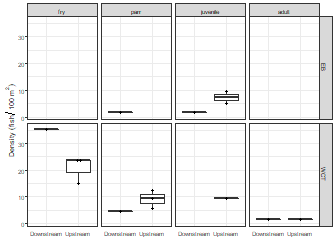
\includegraphics{Elk_files/figure-latex/plot-fish-box-010-1.pdf}
\caption{\label{fig:plot-fish-box-010}Fish densities (fish/100m2) for PSCIS crossing 50155.}
\end{figure}

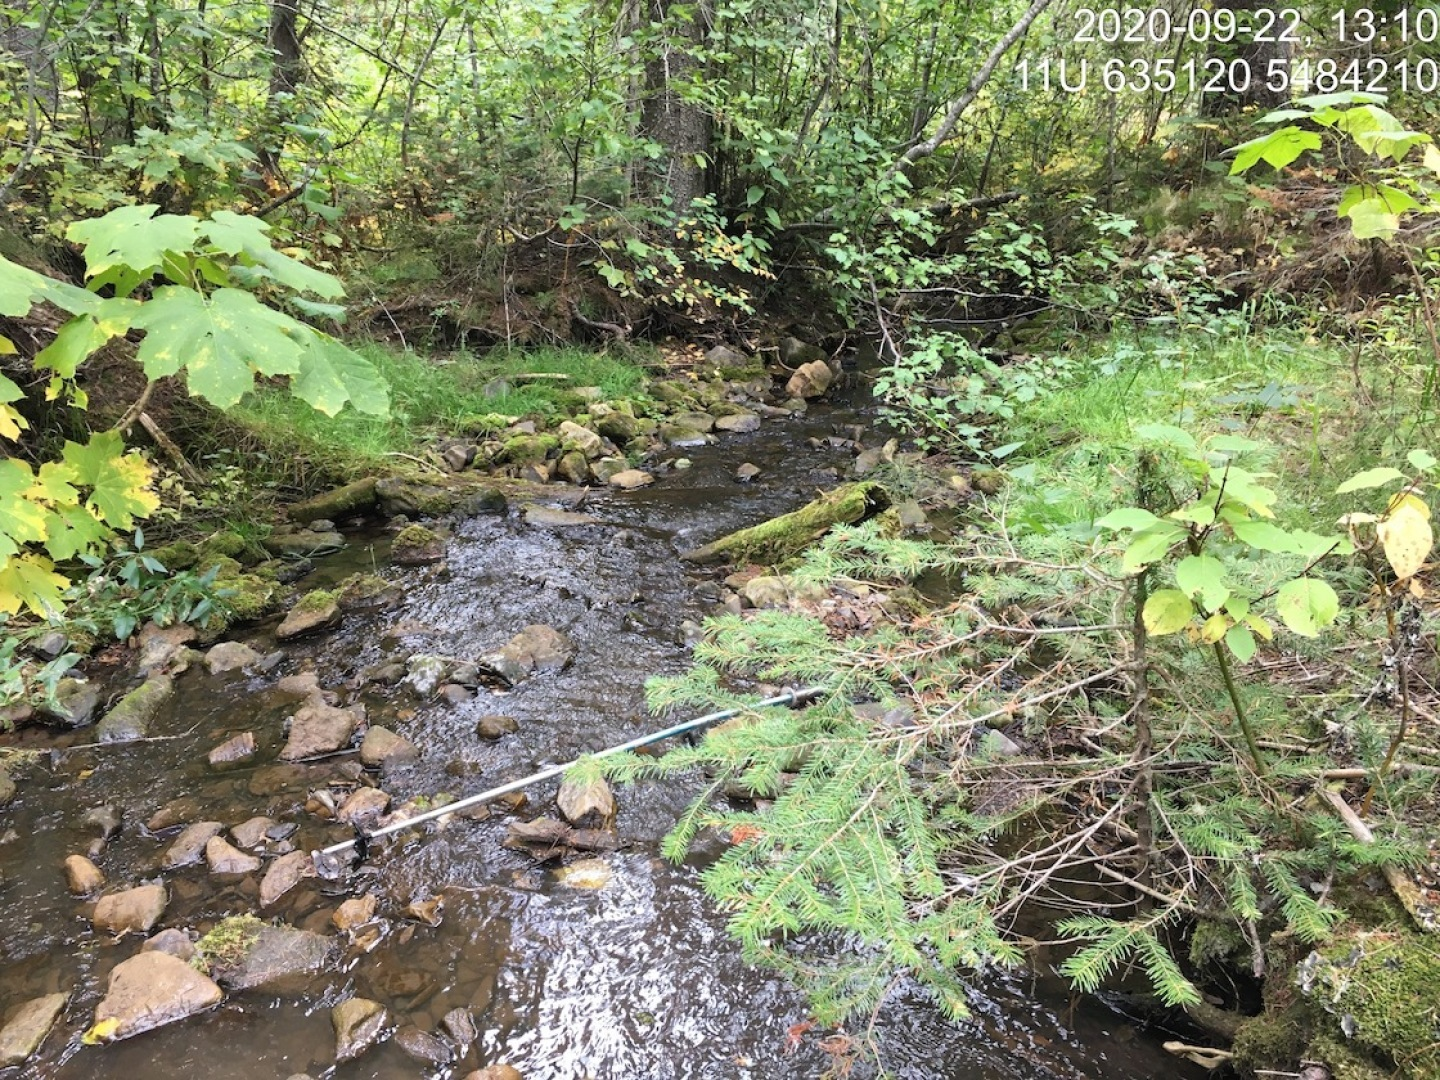
\includegraphics[width=20in]{data/photos/50155/20200922_131045_k}

\begin{figure}
\centering
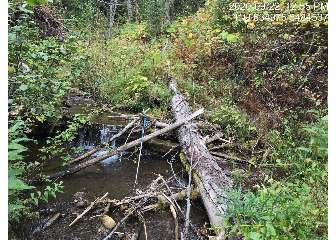
\includegraphics{Elk_files/figure-latex/photo-002-1.pdf}
\caption{\label{fig:photo-002}Typical habitat upstream of PSCIS crossing 50155.}
\end{figure}

  \bibliography{book.bib,packages.bib}

\end{document}
